\documentclass[usenames,dvipsnames,9pt]{beamer}
\usetheme[
    progressbar=frametitle,
    block=fill
  ]{metropolis}


%%%%%%%%%%%%%%%%%%%%%%%%%%%%%%%%%%%%%%%%%%%%%%%%%%%%%%%%%%%%%%%%%%%%%%%%%%%%%%%
% Packages
%%%%%%%%%%%%%%%%%%%%%%%%%%%%%%%%%%%%%%%%%%%%%%%%%%%%%%%%%%%%%%%%%%%%%%%%%%%%%%%

% \usepackage[utf8]{inputenc} % allow utf-8 input
\usepackage{url}            % simple URL typesetting
\usepackage{microtype}      % microtypography
\usepackage{calc}           % perform arithmetic on the arguments
\usepackage{xspace}         % commands that appear not to eat spaces
\usepackage{enumitem}       % control layout of itemize, enumerate
\usepackage{ulem}           % \ul underline command
\usepackage{numprint}       % prints numbers with a separator every three digits
\usepackage{color}          % provides both foreground/background colour management
\usepackage{caption}        % provides many ways to customise the captions in floating environments
\usepackage{subcaption}
\usepackage{lmodern}

\usepackage{copyrightbox}
\usepackage[percent]{overpic}
\usepackage[export]{adjustbox}
\usepackage{mdframed}
\usepackage[super]{nth}
\usepackage[most]{tcolorbox}


% other, check if needed
% \usepackage{xcolor}
% \usepackage[T1]{fontenc}    % use 8-bit T1 fonts
% \usepackage{dsfont} % for mathds{1}
% \usepackage{animate}
% \usepackage{media9}
% \usepackage{makecell}
% \usepackage{graphics}
% \usepackage{relsize}
% \usepackage{fancybox}
% \usepackage[ruled,vlined]{algorithm2e}
% \usepackage{appendixnumberbeamer}
% \usepackage[scale=2]{ccicons}
% \usepackage{fontspec}

% \usefonttheme{professionalfonts} % using non standard fonts for beamer
% \usefonttheme{serif} % default family is serif
% \usepackage{fontspec}
% \setmainfont{Liberation Serif}




%%%%%%%%%%%%%%%%%%%%%%%%%%%%%%%%%%%%%%%%%%%%%%%%%%%%%%%%%%%%%%%%%%%%%%%%%%%%%%%
% Table packages
%%%%%%%%%%%%%%%%%%%%%%%%%%%%%%%%%%%%%%%%%%%%%%%%%%%%%%%%%%%%%%%%%%%%%%%%%%%%%%%

\usepackage{array}          % extending the array and tabular environments
\usepackage{multirow}       % create tabular cells spanning multiple rows
\usepackage{tabularx}       % tabulars with adjustable-width columns
\usepackage{booktabs}       % professional-quality tables

\newcolumntype{P}[1]{>{\centering\arraybackslash}p{#1}}
% \newcolumntype{M}[1]{>{\centering\arraybackslash}m{#1}}

\newsavebox{\mybox}
\newcolumntype{M}[2]{>{\begin{lrbox}{\mybox}}#1<{\end{lrbox}
  \onslide<#2>{\unhbox\mybox}}}


%%%%%%%%%%%%%%%%%%%%%%%%%%%%%%%%%%%%%%%%%%%%%%%%%%%%%%%%%%%%%%%%%%%%%%%%%%%%%%%
% Mathematical packages
%%%%%%%%%%%%%%%%%%%%%%%%%%%%%%%%%%%%%%%%%%%%%%%%%%%%%%%%%%%%%%%%%%%%%%%%%%%%%%%

\usepackage{mathtools}
\usepackage{amsmath}        % Basic mathematical typography
\usepackage{amssymb}
\usepackage{amsthm}         % Basic mathematical environments for proofs etc.
\usepackage{mathdots}       % dots commands for matrices 
\usepackage{amsfonts}       % blackboard math symbols
\usepackage{nicefrac}       % compact symbols for 1/2, etc.
\usepackage{physics}        % typesetting equations for physics simpler

%%%%%%%%%%%%%%%%%%%%%%%%%%%%%%%%%%%%%%%%%%%%%%%%%%%%%%%%%%%%%%%%%%%%%%%%%%%%%%%
% Bibliography
%%%%%%%%%%%%%%%%%%%%%%%%%%%%%%%%%%%%%%%%%%%%%%%%%%%%%%%%%%%%%%%%%%%%%%%%%%%%%%%

\usepackage{bibentry}
\usepackage[round]{natbib}

%%%%%%%%%%%%%%%%%%%%%%%%%%%%%%%%%%%%%%%%%%%%%%%%%%%%%%%%%%%%%%%%%%%%%%%%%%%%%%%
% Graphics packages
%%%%%%%%%%%%%%%%%%%%%%%%%%%%%%%%%%%%%%%%%%%%%%%%%%%%%%%%%%%%%%%%%%%%%%%%%%%%%%%

\usepackage{pgfplots}
% \pgfplotsset{compat=1.14}
\usepackage{tikz}
\usepgfplotslibrary{dateplot}
\usetikzlibrary{positioning}
\usetikzlibrary{arrows.meta}
\usetikzlibrary{arrows,shapes}
\usetikzlibrary{matrix,decorations.pathreplacing,calc}
\usetikzlibrary{decorations.text}
% \usetikzlibrary{external}\tikzexternalize

\usepackage{tikz}
  \tikzset{
    onslide/.code args={<#1>#2}{\only<#1>{\pgfkeysalso{#2}}}, 
  }

\tikzstyle{every picture}+=[remember picture]

\DeclareMathOperator{\Mcol}{col}
\DeclareMathOperator{\Mrow}{row}
\DeclareMathOperator{\Mnull}{null}


%%%%%%%%%%%%%%%%%%%%%%%%%%%%%%%%%%%%%%%%%%%%%%%%%%%%%%%%%%%%%%%%%%%%%%%%%%%%%%%
% Customize template
%%%%%%%%%%%%%%%%%%%%%%%%%%%%%%%%%%%%%%%%%%%%%%%%%%%%%%%%%%%%%%%%%%%%%%%%%%%%%%%

% \setbeamercolor{background canvas}{bg=white}
\setbeamertemplate{frametitle continuation}{}
\setbeamertemplate{theorems}[unnumbered]
\setbeamertemplate{section in toc}[sections numbered]
\setbeamertemplate{subsection in toc}[subsections numbered]

% \AtBeginSubsection[]
% {
% \begin{frame}
%   \frametitle{Table of Contents}
%   \tableofcontents[currentsection,currentsubsection]
% \end{frame}
% }

\renewenvironment{equation}
  {\begin{equation*}}
  {\end{equation*}}


\usefonttheme{professionalfonts} % using non standard fonts for beamer
% \usefonttheme{serif} % default family is serif
% \setmainfont{Liberation Serif}

\definecolor{GreyPSL}{RGB}{100,100,100}
\definecolor{BluePSL}{RGB}{47,68,134}
\definecolor{Pimpalert}{RGB}{128,0,197}
\definecolor{OrangePSL}{RGB}{255,127,0}
\definecolor{SkyBlue}{RGB}{47,68,255}
\definecolor{GrayPSL}{RGB}{67,65,72}
\colorlet{LightBluePSL}{BluePSL!20!}
\definecolor{myred}{RGB}{176, 35, 24}

\definecolor{color1}{RGB}{102, 110, 119}
\definecolor{color2}{RGB}{159, 119,  83}
\definecolor{color3}{RGB}{226, 182, 112}
\definecolor{color4}{RGB}{217, 204, 189}
\definecolor{color5}{RGB}{143, 152, 166}
\definecolor{color6}{RGB}{132, 181, 229}
\definecolor{color7}{RGB}{226, 153,  90}
\definecolor{color8}{RGB}{240, 211, 113}
\definecolor{color9}{RGB}{249, 240, 206}

\definecolor{darkblue}{RGB}{57,119,175}



\setbeamercolor{background canvas}{fg= black!2 , bg=white} 
\setbeamercolor{footline}{fg = normal text.fg, bg = normal text.fg!15! }
\setbeamercolor{beamercolorbox}{fg=white, bg=BluePSL}


%%%%%%%%%%%%%%%%%%%%%%%%%%%%%%%%%%%%%%%%%%%%%%%%%%%%%%%%%%%%%%%%%%%%%%%%%%%%%%%%
% title page
%%%%%%%%%%%%%%%%%%%%%%%%%%%%%%%%%%%%%%%%%%%%%%%%%%%%%%%%%%%%%%%%%%%%%%%%%%%%%%%%

\setbeamertemplate{title page}{
  \begin{minipage}[c][\paperheight]{\textwidth}
    \ifx\inserttitlegraphic\@empty\else\usebeamertemplate*{title graphic}\fi
    \vfill%
    {
      \vspace{-1cm}
      \ifx\inserttitle\@empty\else\usebeamertemplate*{title}\fi
      \ifx\insertsubtitle\@empty\else\usebeamertemplate*{subtitle}\fi
    }
    \usebeamertemplate*{title separator}
    \vspace{12pt}
    \begin{minipage}{\textwidth}
      \begin{flushleft}
	\small{\textbf{Candidate:} Alexandre Araujo \hfill Universit\'e Paris Dauphine -- PSL} \\ [5pt]
	\textbf{Date:} 01/06/2021 \hfill \small{Machine Intelligence and Learning Systems} \\ [7pt]
      \end{flushleft}
    \end{minipage}
    \vspace{1em}

    \begin{minipage}{0.5\textwidth}
      \textbf{PhD advisors:}
      \footnotesize{
	\begin{itemize}[itemsep=0pt]
	  \item Jamal Atif
	  \item Yann Chevaleyre
	  \item Benjamin Negrevergne
	  \item \phantom{test}
	  \item \phantom{test}
	\end{itemize}
      }
    \end{minipage}
    \begin{minipage}{0.51\textwidth}
      \textbf{Jury members:}
      \footnotesize{
	\begin{itemize}[itemsep=0pt]
	  \item Teddy Furon (Reviewer)
	  \item Alain Rakotomamonjy (Reviewer)
	  \item Rémi Gribonval (Examiner)
	  \item Elisa Fromont (Examiner)
	  \item Krzysztof Choromanski (Examiner)
	\end{itemize}
      }
    \end{minipage}
    \vfill
    \vspace{1pt}
  \end{minipage}
}




\makeatletter
\setlength{\metropolis@titleseparator@linewidth}{0.5pt}
\setlength{\metropolis@progressonsectionpage@linewidth}{1.2pt}
\setlength{\metropolis@progressinheadfoot@linewidth}{1.2pt}
\makeatother


%%%%%%%%%%%%%%%%%%%%%%%%%%%%%%%%%%%%%%%%%%%%%%%%%%%%%%%%%%%%%%%%%%%%%%%%%%%%%%%%
% footer
%%%%%%%%%%%%%%%%%%%%%%%%%%%%%%%%%%%%%%%%%%%%%%%%%%%%%%%%%%%%%%%%%%%%%%%%%%%%%%%%

\setbeamertemplate{frame footer}{
~~\textbf{Alexandre Araujo - PhD Defense} \hfill \tiny{Building Compact and Robust Deep Neural Networks with Toeplitz Matrices}}

\makeatletter
\setbeamertemplate{footline}{%
  \begin{center}
    \rule{1.2\linewidth}{0.3pt}
  \end{center}
  \vspace{-6pt}
  \begin{beamercolorbox}[wd=\textwidth, sep=1ex]{footline}
    \usebeamerfont{page number in head/foot}%
    \usebeamertemplate*{frame footer}
    \hfill%
    \usebeamertemplate*{frame numbering} 
      ~~\raisebox{-1.3ex}{\includegraphics[height=4ex]{logos/psl.png}}~~
  \end{beamercolorbox}%
}
\makeatother


%%%%%%%%%%%%%%%%%%%%%%%%%%%%%%%%%%%%%%%%%%%%%%%%%%%%%%%%%%%%%%%%%%%%%%%%%%%%%%%%
% custom command
%%%%%%%%%%%%%%%%%%%%%%%%%%%%%%%%%%%%%%%%%%%%%%%%%%%%%%%%%%%%%%%%%%%%%%%%%%%%%%%%

\renewcommand{\bibsection}{}
% \newtheorem{proposition}{Proposition}[section]
\newcommand{\yt}{\textit{YouTube-8M}\xspace}
\newcommand{\eg}{\textit{e.g.}\xspace}
\newcommand{\ie}{\textit{i.e.}\xspace}

\newcommand{\ci}{\mathbf{i}}

\DeclareMathOperator*{\lip}{Lip}
\DeclareMathOperator*{\lipbound}{LipBound}

\newcommand{\seqidx}{h}
\newcommand{\seqsetN}{N}
\newcommand{\seqsetM}{M}

% cin et cout
\newcommand{\cin}{\ensuremath{\mathrm{cin}}}
\newcommand{\cout}{\ensuremath{\mathrm{cout}}}

\DeclareMathOperator*{\argmax}{arg\,max}
\DeclareMathOperator*{\argmin}{arg\,min}
\DeclareMathOperator*{\E}{\Ebb}

% norms
\newcommand{\lone}{\ensuremath \ell_1}
\newcommand{\ltwo}{\ensuremath \ell_2}
\newcommand{\linf}{\ensuremath \ell_\infty}


\def\ddefloop#1{\ifx\ddefloop#1\else\ddef{#1}\expandafter\ddefloop\fi}

% domains
\def\ddef#1{\expandafter\def\csname #1bb\endcsname{\ensuremath{\mathbb{#1}}}}
\ddefloop ABCDEFGHIJKLMNOPQRSTUVWXYZ\ddefloop
% sets
\def\ddef#1{\expandafter\def\csname #1cal\endcsname{\ensuremath{\mathcal{#1}}}}
\ddefloop ABCDEFGHIJKLMNOPQRSTUVWXYZ\ddefloop
% bold matrices
\def\ddef#1{\expandafter\def\csname #1mat\endcsname{\ensuremath{\mathbf{#1}}}}
\ddefloop ABCDEFGHIJKLMNOPQRSTUVWXYZ\ddefloop
% sans serif matrices
\def\ddef#1{\expandafter\def\csname #1matsf\endcsname{\ensuremath{\mathsf{#1}}}}
\ddefloop ABCDEFGHIJKLMNOPQRSTUVWXYZ\ddefloop
% bold vectors
\def\ddef#1{\expandafter\def\csname #1vec\endcsname{\ensuremath{\mathbf{#1}}}}
\ddefloop abcdefghijklmnopqrstuvwxyz\ddefloop


% sans sherif
\def\ddef#1{\expandafter\def\csname #1sf\endcsname{\ensuremath{\mathsf{#1}}}}
\ddefloop abcdefghijklmnopqrstuvwxyz\ddefloop
% sans sherif
\def\ddef#1{\expandafter\def\csname #1sf\endcsname{\ensuremath{\mathsf{#1}}}}
\ddefloop ABCDEFGHIJKLMNOPQRSTUVWXYZ\ddefloop

% bold sans sherif
\def\ddef#1{\expandafter\def\csname #1bsf\endcsname{\ensuremath{\boldsymbol{\mathsf{#1}}}}}
\ddefloop abcdefghijklmnopqrstuvwxyz\ddefloop
% bold sans sherif
\def\ddef#1{\expandafter\def\csname #1bsf\endcsname{\ensuremath{\boldsymbol{\mathsf{#1}}}}}
\ddefloop ABCDEFGHIJKLMNOPQRSTUVWXYZ\ddefloop

% special command for big O notation
\newcommand{\bigO}{\ensuremath \mathcal{O}}

% matrix brackets
\newcommand{\leftmatrix}{\begin{pmatrix}}
\newcommand{\rightmatrix}{\end{pmatrix}}
\newcommand{\leftmat}{\left(}
\newcommand{\rightmat}{\right)}

% circulant & diagonal
\newcommand{\circulant}{\ensuremath \mathrm{circ}}
\newcommand{\diagonal}{\ensuremath \mathrm{diag}}

\newcommand{\orange}[1]{{\color{OrangePSL}{#1}}}
\newcommand{\orangebold}[1]{{\color{OrangePSL}{\textbf{#1}}}}



%%%%%%%%%%%%%%%%%%%%%%%%%%%%%%%%%%%%%%%%%%%%%%%%%%%%%%%%%%%%%%%%%%%%%%%%%%%%%%%
% Debugging
%%%%%%%%%%%%%%%%%%%%%%%%%%%%%%%%%%%%%%%%%%%%%%%%%%%%%%%%%%%%%%%%%%%%%%%%%%%%%%%

\newcommand{\todo}[1]{\textcolor{red}{\textbf{TODO:} #1\xspace}}





\title{\normalsize{Compact and Robust Deep Neural Networks with Toeplitz Matrices}}
\subtitle{\normalsize{A structured matrix approach to Deep Learning}}
\date{01/06/2021}
\author{Alexandre Araujo}
\institute{Universit\'e Paris-Dauphine-PSL}

\titlegraphic{
  \vspace{22em}
  \begin{minipage}{\textwidth}
    \centering
    % \begin{column}{.18\textwidth}
    %   \fbox{
\includegraphics[trim={0 5cm 0 5cm}, clip, width=2cm]{logos/PSL.png}
    %   }
    % \end{column}
    \begin{minipage}{.26\textwidth}
      
\includegraphics[trim={0.1cm 0 0.2cm 0},clip,scale=0.08]{logos/Dauphine_logo_2019.png}
    \end{minipage}
    \begin{minipage}{.22\textwidth}
      \centering
      
\includegraphics[scale=0.15]{logos/lamsade.jpg}
    \end{minipage}
    \begin{minipage}{.12\textwidth}
      \centering
      
\includegraphics[trim={0.6cm 1.3cm 1.3cm 0.3cm},clip,scale=0.1]{logos/logomiles_small.pdf}
    \end{minipage}
    \begin{minipage}{.1\textwidth}
      \centering
      
\includegraphics[scale=0.02]{logos/cnrs.png}
    \end{minipage}
    \begin{minipage}{.22\textwidth}
      \centering
      
\includegraphics[trim={3.1cm 0 3.7cm 0},clip,scale=0.05]{logos/wavestone.png}
    \end{minipage}
  \end{minipage}
}


%%%%%%%%%%%%%%%%%%%%%%%%%%%%%%%%%%%%%%%%%%%%%%%%%%%%%%%%%%%%%%%%%%%%%%%%%%%%%%%
% Document
%%%%%%%%%%%%%%%%%%%%%%%%%%%%%%%%%%%%%%%%%%%%%%%%%%%%%%%%%%%%%%%%%%%%%%%%%%%%%%%

\begin{document}

  \maketitle

  %%%%%%%%%%%%%%%%%%%%%%%%%%%%%%%%%%%%%%%%%%%%%%%%%%%%%%%%%%%%%%%%%%%%%%%%%%%%%%%
\section{Context \& Background}
%%%%%%%%%%%%%%%%%%%%%%%%%%%%%%%%%%%%%%%%%%%%%%%%%%%%%%%%%%%%%%%%%%%%%%%%%%%%%%%


%%%%%%%%%%%%%%%%%%%%%%%%%%%%%%%%%%%%%%%%%%%%%%%%%%%%%%%%%%%%%%%%%%%%%%%%%%%%%%%
\begin{frame}{Supervised Learning Algorithms}
%%%%%%%%%%%%%%%%%%%%%%%%%%%%%%%%%%%%%%%%%%%%%%%%%%%%%%%%%%%%%%%%%%%%%%%%%%%%%%%
  \begin{figure}
    \begin{minipage}[!ht]{0.42\textwidth}
      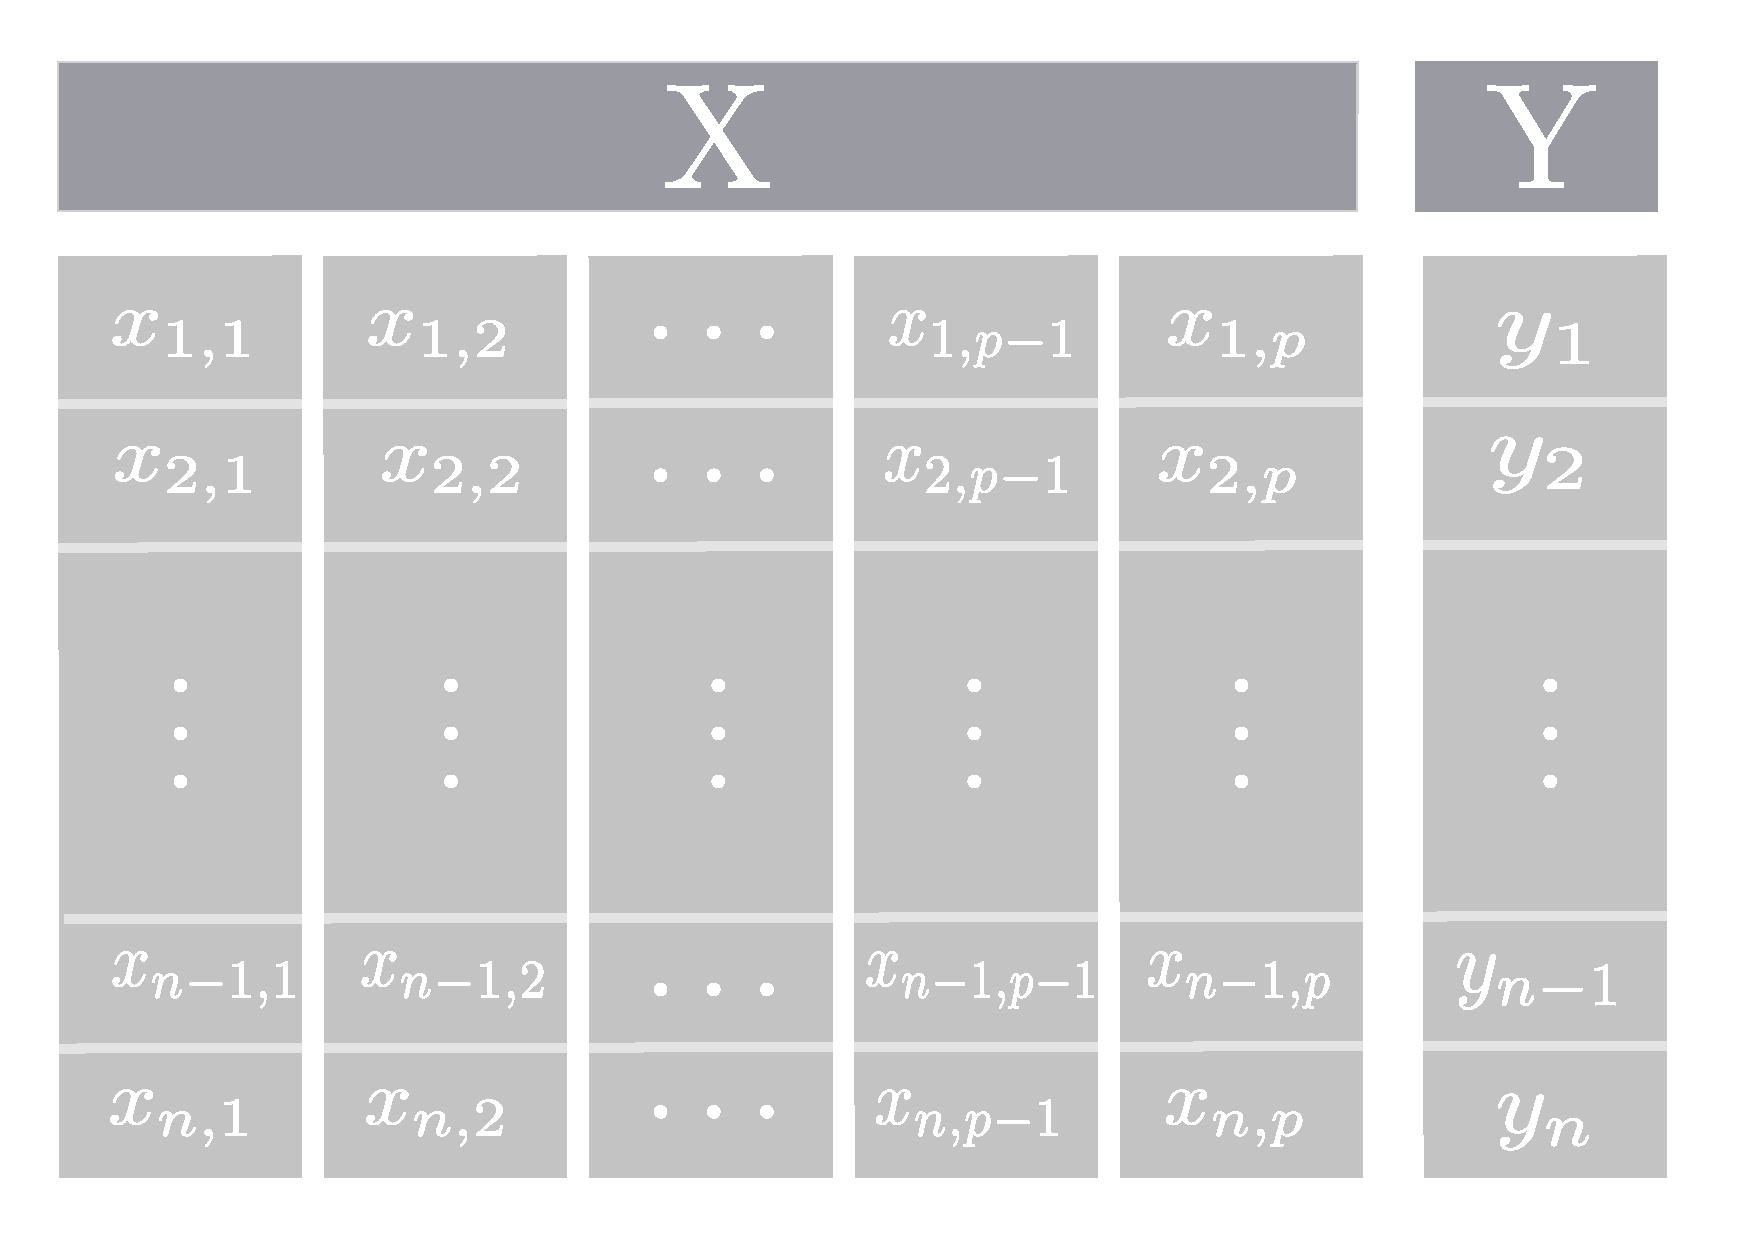
\includegraphics[width=\textwidth]{images/TableauDonneeApprentissage.pdf}
    \end{minipage} \hspace{0.3cm}
    \begin{minipage}[!ht]{0.52\textwidth}
      Given a set of $n$ \textbf{training examples} $\left\{ (\xvec_1, y_1),\dots,(\xvec_n, y_n) \right\}$ where $\xvec_i$ is the feature vector of the $i^{th}$ example, and $y_i$ is the corresponding label. \\
      \textbf{Assumption:} there is a function $f$ matching any feature vector to its label.
   \end{minipage}
  \end{figure}
    The goal of a \textbf{learning algorithm} is to approximate $f$ by a parameterized function $f_\theta$.
    In order to measure how well the function fits, \textbf{a loss function} $\mathcal{L}: \mathcal{Y} \times \mathcal{Y} \rightarrow \Rbb^{+}$ is defined.
    The standard method to learn the set of parameters $\theta$ is the \textbf{empirical risk minimization (ERM)}:
  \begin{equation*}
    \hat{\theta}_{ERM} \triangleq \argmin_{\theta} \frac{1}{n} \sum_{i=1}^{n} \mathcal{L} (f_{\theta} (\xvec_i), y_i )
  \end{equation*}
\end{frame}



%%%%%%%%%%%%%%%%%%%%%%%%%%%%%%%%%%%%%%%%%%%%%%%%%%%%%%%%%%%%%%%%%%%%%%%%%%%%%%%
\begin{frame}{Deep neural networks}
%%%%%%%%%%%%%%%%%%%%%%%%%%%%%%%%%%%%%%%%%%%%%%%%%%%%%%%%%%%%%%%%%%%%%%%%%%%%%%%

  Neural Neural can be analytically described as a composition of linear functions interlaced with non-linear functions:
  \begin{block}{Neural Network}
      A neural network of $\ell$ layers is defined as follows:
      \begin{equation*}
	\mathcal{N}_\theta(\xvec) = \phi_{\Wmat_\ell,\bvec_\ell} \circ \rho \circ \phi_{\Wmat_{\ell-1}, \bvec_{\ell-1}} \circ \rho \circ \cdots \circ \rho \circ \phi_{\Wmat_1, \bvec_1}(\xvec)
      \end{equation*}
      where for any $i$, $\phi_{\Wmat_i,\bvec_i} \triangleq \xvec \mapsto \Wmat_i \xvec + \bvec_i$, $\xvec_i \in \Rbb^n$, $\bvec_i \in \Rbb^m$, $\Wmat_i \in \Rbb^{m \times n}$, $\rho$ some non linear functions and $\theta$ corresponds to the set of all parameters.
  \end{block}

  \begin{block}{Evaluation of Neural Networks}
    \begin{itemize}
      \item[$\bullet$] Classical evaluation with accuracy
      \item[$\bullet$] Robust evaluation against adversarial attacks
    \end{itemize}
  \end{block}

\end{frame}


%%%%%%%%%%%%%%%%%%%%%%%%%%%%%%%%%%%%%%%%%%%%%%%%%%%%%%%%%%%%%%%%%%%%%%%%%%%%%%%
\begin{frame}{Adversarial Attacks}
%%%%%%%%%%%%%%%%%%%%%%%%%%%%%%%%%%%%%%%%%%%%%%%%%%%%%%%%%%%%%%%%%%%%%%%%%%%%%%%
  An \textbf{adversarial attack} refers to a small, imperceptible change of an input maliciously designed to fool the result of a machine learning algorithm. 
  \begin{center}
    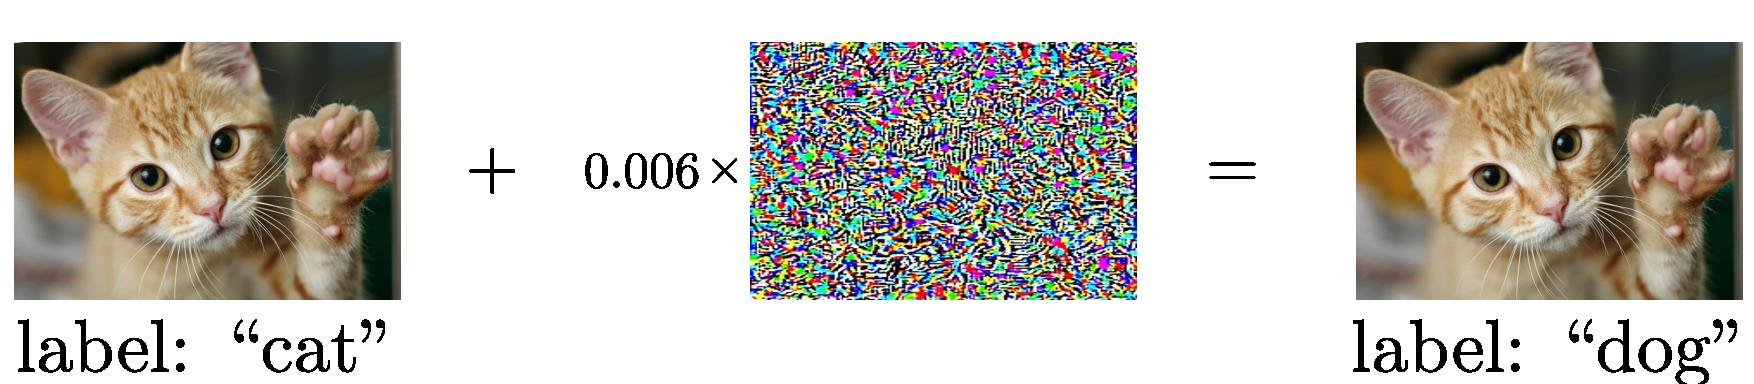
\includegraphics[width=\textwidth]{images/ExampleAdversarialCatDog.pdf}
  \end{center}
  Since the seminal work of \cite{Szegedy2013IntriguingPO}, numerous attack methods have been designed:
  \begin{itemize}
    \item[$\bullet$] \textbf{PGD} \cite{madry2018towards}
    \item[$\bullet$] \textbf{C\&W} \cite{carlini2017towards}
  \end{itemize}

\end{frame}


% %%%%%%%%%%%%%%%%%%%%%%%%%%%%%%%%%%%%%%%%%%%%%%%%%%%%%%%%%%%%%%%%%%%%%%%%%%%%%%%
% \begin{frame}{Adversarial Attacks}
% %%%%%%%%%%%%%%%%%%%%%%%%%%%%%%%%%%%%%%%%%%%%%%%%%%%%%%%%%%%%%%%%%%%%%%%%%%%%%%%
%
%   Given an input-output pair $(\xvec, y) \sim \mathcal{D}$, an \textbf{adversarial attack} is a procedure that produces a small perturbation $\mathbf{\tau} \in \mathcal{X}$ such that $\mathcal{N}_\theta(\xvec + \mathbf{\tau}) \neq y$.
%
%   Existing attacks can adopt one of the two following strategies:
%   \begin{itemize}
%     \item[1.] maximizing the loss $\mathcal{L}(\mathcal{N}_\theta(\xvec + \tau), y)$ under some constraint on $\norm{\tau}_p$;
%     \item[2.] minimizing $\norm{\tau}_p$ under some constraint on the loss $\mathcal{L}(\mathcal{N}_\theta(\xvec + \tau), y)$;
%   \end{itemize}
%
%   In the following, we will use:
%   \begin{itemize}
%     \item Strategy 1: \textbf{PGD}-$\ell_\infty$ attack (\cite{madry2018towards})
%     \item Strategy 2: \textbf{C\&W}-$\ell_2$ attack (\citet{carlini2017towards})
%   \end{itemize}
%
% \end{frame}



%%%%%%%%%%%%%%%%%%%%%%%%%%%%%%%%%%%%%%%%%%%%%%%%%%%%%%%%%%%%%%%%%%%%%%%%%%%%%%%
\begin{frame}{Limits of Large Neural Networks}
%%%%%%%%%%%%%%%%%%%%%%%%%%%%%%%%%%%%%%%%%%%%%%%%%%%%%%%%%%%%%%%%%%%%%%%%%%%%%%%

  Fully-Connected Neural Networks (neural networks defined with dense matrices) can have a \emph{very large number of parameters}.

  $\Rightarrow$ With MNIST dataset (\cite{lecun1998gradient}), a two-layers Fully-Connected neural network will have more than $\mathbf{6 \times 10^5}$ \textbf{parameters}.

  \vspace{0.5cm}

  \begin{block}{Limits of Large Neural Networks}
    \begin{itemize}
      \small
      \item[$\bullet$] They are hard to train
      \item[$\bullet$] They are subject to overfitting: they don't generalize well
      \item[$\bullet$] They are computationally expensive 
    \end{itemize}
  \end{block}
  
  $\Rightarrow$ To overcome these limitations, researchers have devised neural networks with \textbf{structured linear operations} in order to reduce the number of parameters needed.

\end{frame}



%%%%%%%%%%%%%%%%%%%%%%%%%%%%%%%%%%%%%%%%%%%%%%%%%%%%%%%%%%%%%%%%%%%%%%%%%%%%%%%
\begin{frame}{Structured matrices for Deep Neural Networks}
%%%%%%%%%%%%%%%%%%%%%%%%%%%%%%%%%%%%%%%%%%%%%%%%%%%%%%%%%%%%%%%%%%%%%%%%%%%%%%%

  A $n \times n$ structured matrix can be represented with less than $n^2$ parameters. In addition to offering a more compact representation, the structure of certain matrices can be leveraged to obtain better algorithms for matrix-vector product.

  \begin{figure}[ht]
     \centering
     \begin{subfigure}[t]{2.2cm}
	 \centering
	 \begin{equation*}
	   \begin{pmatrix}
	      a &   &   &   \\
		& b &   &   \\
		&   & c &   \\
		&   &   & d
	   \end{pmatrix}
	 \end{equation*}
	 \caption*{diagonal}
     \end{subfigure}
     \begin{subfigure}[t]{2.2cm}
	 \centering
	 \begin{equation*}
	    \begin{pmatrix}
	      a & b & c & d \\
	      e & a & b & c \\
	      f & e & a & b \\
	      d & f & e & a
	    \end{pmatrix}
	 \end{equation*}
	 \caption*{Toeplitz}
     \end{subfigure}
     \begin{subfigure}[t]{2.8cm}
	 \centering
	 \begin{equation*}
	    \begin{pmatrix}
	      ae & af & ag & ah \\
	      be & bf & bg & bh \\
	      ce & cf & cg & ch \\
	      de & df & dg & dh
	    \end{pmatrix}
	 \end{equation*}
	 \caption*{Low Rank}
     \end{subfigure}
     \begin{subfigure}[t]{2.8cm}
	 \centering
	 \begin{equation*}
	    \begin{pmatrix}
	      a & a^2 & a^3 & a^4 \\
	      b & b^2 & b^3 & b^4 \\
	      c & c^2 & c^3 & c^4 \\
	      d & d^2 & d^3 & d^4
	    \end{pmatrix}
	 \end{equation*}
	 \caption*{Vandermonde}
     \end{subfigure}
    \caption{Examples of structured matrices.}
    \label{figure:example_structure_matrices}
  \end{figure}

  $\Rightarrow$ We focus on structured matrices from the \textbf{Toeplitz family}. 

\end{frame}


%%%%%%%%%%%%%%%%%%%%%%%%%%%%%%%%%%%%%%%%%%%%%%%%%%%%%%%%%%%%%%%%%%%%%%%%%%%%%%%
\begin{frame}{Focus on structured matrices from the Toeplitz family}
%%%%%%%%%%%%%%%%%%%%%%%%%%%%%%%%%%%%%%%%%%%%%%%%%%%%%%%%%%%%%%%%%%%%%%%%%%%%%%%
  More specifically:
  A Toeplitz matrix is a matrix with constant diagonal:
  \begin{figure}
    \begin{subfigure}[b]{0.3\textwidth}
     \centering
     \begin{equation*}
	\begin{pmatrix}
	  a & b & c & d \\
	  e & a & b & c \\
	  f & e & a & b \\
	  d & f & e & a
	\end{pmatrix}
     \end{equation*}
     \caption*{}
    \end{subfigure}
    \hfill
    \begin{subfigure}[b]{0.3\textwidth}
      \centering
      
\includegraphics[width=0.65\textwidth]{images/toeplitz_v1.pdf}
      \caption*{}
    \end{subfigure}
    \hfill
    \begin{subfigure}[b]{0.3\textwidth}
      \centering
      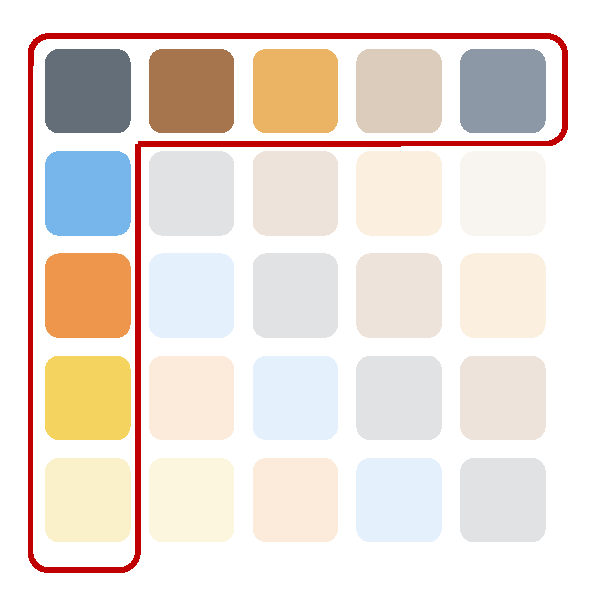
\includegraphics[width=0.65\textwidth]{images/toeplitz_v2.pdf}
      \caption*{}
    \end{subfigure}
  \end{figure}

  $\Rightarrow$ A $n \times n$ Toeplitz matrix has $2n - 1$ unique values. 

  % $\Rightarrow$ We can constraint or generalize the Toeplitz structure.

\end{frame}



%%%%%%%%%%%%%%%%%%%%%%%%%%%%%%%%%%%%%%%%%%%%%%%%%%%%%%%%%%%%%%%%%%%%%%%%%%%%%%%
\begin{frame}{Focus on structured matrices from the Toeplitz family}
%%%%%%%%%%%%%%%%%%%%%%%%%%%%%%%%%%%%%%%%%%%%%%%%%%%%%%%%%%%%%%%%%%%%%%%%%%%%%%%
  
  For our contributions, we study:
  \begin{itemize}
    \item[$\bullet$] Circulant matrices
    \item[$\bullet$] Doubly-block Toeplitz matrices
  \end{itemize}

\end{frame}


%%%%%%%%%%%%%%%%%%%%%%%%%%%%%%%%%%%%%%%%%%%%%%%%%%%%%%%%%%%%%%%%%%%%%%%%%%%%%%%
\begin{frame}{Circulant Matrices}
%%%%%%%%%%%%%%%%%%%%%%%%%%%%%%%%%%%%%%%%%%%%%%%%%%%%%%%%%%%%%%%%%%%%%%%%%%%%%%%

  A $n \times n$ circulant matrix is a matrix where each row is a cyclic right shift of the previous one. 

  % \begin{figure}
  %   \begin{subfigure}[b]{0.3\textwidth}
  %     \centering
  %     
\includegraphics[width=0.65\textwidth]{images/circulant_v1.pdf}
  %     \caption*{A circulant matrix}
  %   \end{subfigure}
  %   \hfill
  %   \begin{subfigure}[b]{0.3\textwidth}
  %     \centering
  %     
\includegraphics[width=0.65\textwidth]{images/circulant_v2.pdf}
  %     \caption*{First row of a  circulant matrix}
  %   \end{subfigure}
  %   \hfill
  %   \begin{subfigure}[b]{0.3\textwidth}
  %     \centering
  %     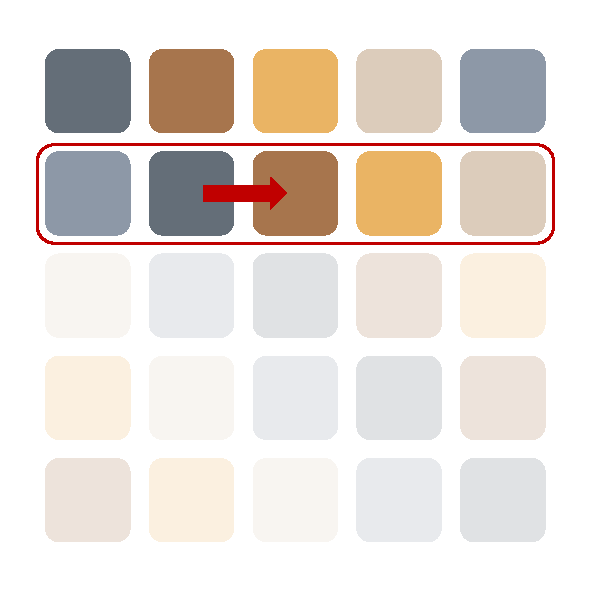
\includegraphics[width=0.65\textwidth]{images/circulant_v3.pdf}
  %     \caption*{First row, shifted on the right}
  %   \end{subfigure}
  % \end{figure}
  
  
  \begin{figure}
    \centering
    
\includegraphics[width=0.35\textwidth]{images/circulant_v1.pdf}
    \caption*{A circulant matrix}
  \end{figure}

\end{frame}


%%%%%%%%%%%%%%%%%%%%%%%%%%%%%%%%%%%%%%%%%%%%%%%%%%%%%%%%%%%%%%%%%%%%%%%%%%%%%%%
\begin{frame}{Doubly-Block Toeplitz Matrices}
%%%%%%%%%%%%%%%%%%%%%%%%%%%%%%%%%%%%%%%%%%%%%%%%%%%%%%%%%%%%%%%%%%%%%%%%%%%%%%%

  A block Toeplitz matrix is a matrix which contains \textbf{blocks that are repeated down the diagonals} of the matrix.

  A \textbf{doubly-block Toeplitz matrix} is a block Toeplitz matrix where all blocks are also Toeplitz.

  \begin{figure}
    \centering
    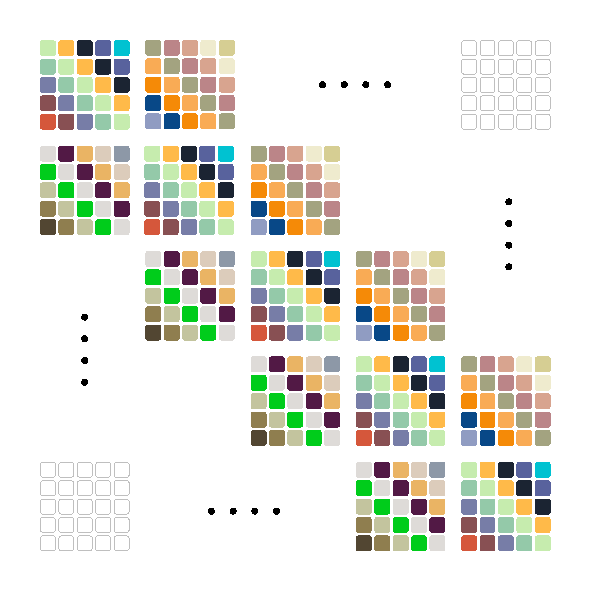
\includegraphics[width=0.35\textwidth]{images/doubly_block.pdf}
    \caption*{Doubly-block Toeplitz matrices}
  \end{figure}

  $\Rightarrow$ Doubly-block matrices are equivalent to the 2d convolution.
  
\end{frame}






% %%%%%%%%%%%%%%%%%%%%%%%%%%%%%%%%%%%%%%%%%%%%%%%%%%%%%%%%%%%%%%%%%%%%%%%%%%%%%%%
% \begin{frame}{Convolutional Neural Networks}
% %%%%%%%%%%%%%%%%%%%%%%%%%%%%%%%%%%%%%%%%%%%%%%%%%%%%%%%%%%%%%%%%%%%%%%%%%%%%%%%
%   Convolutional Neural Networks are state-of-the-art for image classification.
%   \begin{figure}
%     \centering
%     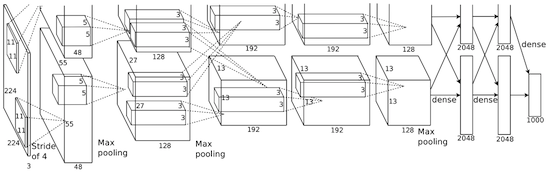
\includegraphics[width=0.8\textwidth]{images/alexnet.png}
%     \caption{Architecture of AlexNet \cite{}}
%   \end{figure}
%   Convolutional Neural Networks use a specific \textbf{structure as linear operations}. 
% \end{frame}


% %%%%%%%%%%%%%%%%%%%%%%%%%%%%%%%%%%%%%%%%%%%%%%%%%%%%%%%%%%%%%%%%%%%%%%%%%%%%%%%
% \begin{frame}{Convolution as matrix-multiplication}
% %%%%%%%%%%%%%%%%%%%%%%%%%%%%%%%%%%%%%%%%%%%%%%%%%%%%%%%%%%%%%%%%%%%%%%%%%%%%%%%
%
%   A discrete convolution between a signal $\xvec$ and a kernel $\kvec$ can be expressed as a product between the vectorization of $\xvec$ and a doubly-block Toeplitz matrix $\Mmat$, whose coefficients have been chosen to match the convolution $\xvec * \kvec$.
%
%   \begin{figure}
%     \begin{subfigure}[t]{0.49\textwidth}
%       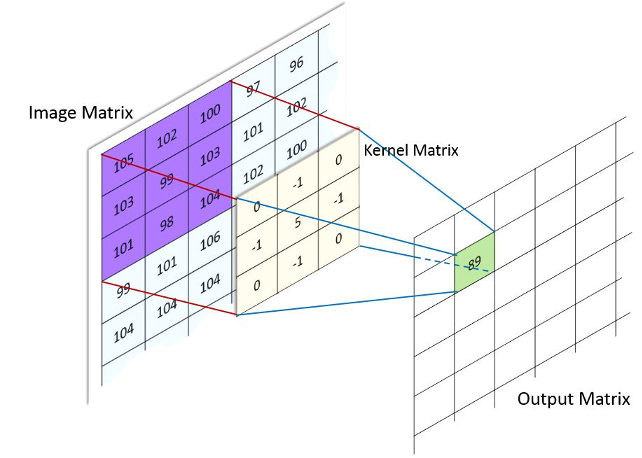
\includegraphics[width=\textwidth]{images/convolution.png}
%       \caption*{Convolution between an 2 dimensional image and a 2 dimensional kernel}
%     \end{subfigure}
%     \begin{subfigure}[t]{0.45\textwidth}
%       \centering
%       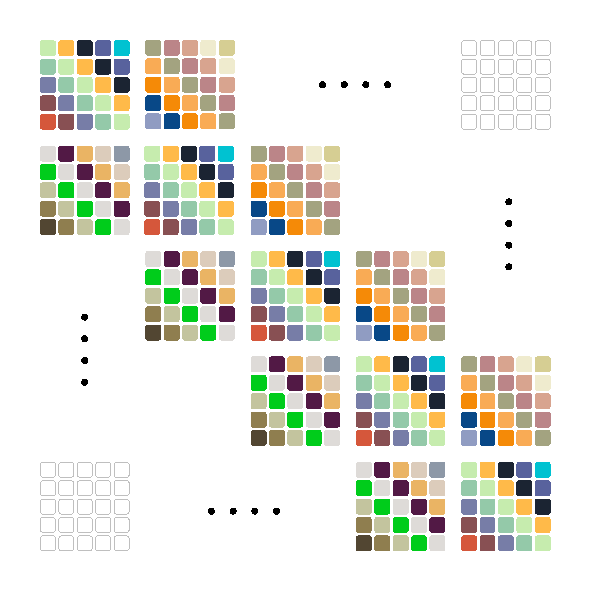
\includegraphics[width=0.8\textwidth]{images/doubly_block.pdf}
%       \caption*{Representation of a Doubly-Block Toeplitz matrix}
%     \end{subfigure}
%   \end{figure}
%
%   When the images has multiples \textit{feature maps}, the matrix $\Mmat$ is the concatenation of multiple Doubly-block Toeplitz matrices.
%   
% \end{frame}


%%%%%%%%%%%%%%%%%%%%%%%%%%%%%%%%%%%%%%%%%%%%%%%%%%%%%%%%%%%%%%%%%%%%%%%%%%%%%%%
\begin{frame}{Our Contributions}
%%%%%%%%%%%%%%%%%%%%%%%%%%%%%%%%%%%%%%%%%%%%%%%%%%%%%%%%%%%%%%%%%%%%%%%%%%%%%%%

  \begin{block}{We devised a compact architecture with Diagonal and Circulant Matrices}
    \begin{itemize}[leftmargin=*]
      \item[] {\small We define the expressive power of diagonal circulant neural networks.}
      \item[] {\small We use diagonal circulant neural networks for compact large scale video classification.}
    \end{itemize}
  \end{block}

  \begin{block}{Improving Robustness of Convolution Neural Networks with Doubly-Block Toeplitz matrices}
    \begin{itemize}[leftmargin=*]
      \item[] {\small We devise an upper bound on the singular values of convolutional layers.}
      \item[] {\small We propose an efficient algorithm to compute this upper bound.}
      \item[] {\small We propose a new regularization scheme to improve the robustness of Neural Networks.}
    \end{itemize}
  \end{block}

\end{frame}




  % %%%%%%%%%%%%%%%%%%%%%%%%%%%%%%%%%%%%%%%%%%%%%%%%%%%%%%%%%%%%%%%%%%%%%%%%%%%%%%%
\section{\orangebold{Part 1.} Compact Neural Networks with Diagonal and Circulant Matrices}
%%%%%%%%%%%%%%%%%%%%%%%%%%%%%%%%%%%%%%%%%%%%%%%%%%%%%%%%%%%%%%%%%%%%%%%%%%%%%%%



%%%%%%%%%%%%%%%%%%%%%%%%%%%%%%%%%%%%%%%%%%%%%%%%%%%%%%%%%%%%%%%%%%%%%%%%%%%%%%%
\begin{frame}{Circulant matrices for Deep Learning}
%%%%%%%%%%%%%%%%%%%%%%%%%%%%%%%%%%%%%%%%%%%%%%%%%%%%%%%%%%%%%%%%%%%%%%%%%%%%%%%

  Recall the Fully-Connected layer:
  \begin{equation}
    \xvec \mapsto \rho\left( {\color<2->{OrangePSL}{\Wmat}} \xvec + \bvec \right)
  \end{equation}

  \vspace{-0.4cm}
  where $\Wmat \in \Rbb^{n \times n}$, $\bvec \in \Rbb^n$.

  \vspace{0.3cm}
  \visible<2->{
    \begin{mdframed}[linecolor=OrangePSL,linewidth=1pt]
      \centering
      % \textbf{Goal}: We want to reduce the number of parameters of the layer. \\
       Can we replace the dense matrix $\Wmat$ with a structured one ? 
    \end{mdframed}
  } 
   
  \vspace{0.3cm}
  \visible<3->{
    Circulant matrices have numerous advantages:
    \begin{itemize}
	\item[$\bullet$] <3-> A circulant matrix can be \orangebold{compactly represented in memory};
	\item[$\bullet$] <3-> The matrix-vector product with a circulant matrix \orangebold{can be done efficiently in the Fourier domain}
        \item[$\Rightarrow$] <4-> They are not expressive: circulant matrices are closed under product.
    \end{itemize}
  }


\end{frame}



%%%%%%%%%%%%%%%%%%%%%%%%%%%%%%%%%%%%%%%%%%%%%%%%%%%%%%%%%%%%%%%%%%%%%%%%%%%%%%%
\begin{frame}{Expressivity of the product of diagonal and circulant matrices}
%%%%%%%%%%%%%%%%%%%%%%%%%%%%%%%%%%%%%%%%%%%%%%%%%%%%%%%%%%%%%%%%%%%%%%%%%%%%%%%

  \begin{minipage}{\textwidth}
    \centering
    Combining circulant matrices with \orangebold{diagonal matrices} improve the expressivity.
  \end{minipage}
  \vspace{0.05cm}

  \visible<2->{
    \begin{theorem}[Reformulation from {\color{SkyBlue}{\citet{huhtanen2015factoring}}}] 
      For every matrix $\Amat \in \Cbb^{n \times n}$, for any $\epsilon > 0$, there exists a sequence of circulant matrices and a sequence of diagonal matrices such that 
      \begin{equation}
	\norm{\prod_{i=1}^{n+1} \Dmat^{(i)} \Cmat^{(i)} - \Amat}_{\mathrm{F}} < \epsilon \enspace.
      \end{equation}
    \end{theorem}
  }

  {\small
  \visible<3->{\textbf{Advantages}}
  \begin{itemize}[parsep=0pt,leftmargin=15pt]
    \nointerlineskip
    \item[$\bullet$] <3-> Neural networks with Diagonal and Circulant Layer are \textbf{universal approximators}; 
  \end{itemize}

  \visible<4->{\textbf{Limits}}
  \begin{itemize}[parsep=0pt,leftmargin=15pt]
    \nointerlineskip
    \item[$\bullet$] <4-> The decomposition needs more values that $n^2$
    \item[$\bullet$] <5-> The theorem does not provide any insights regarding the expressive power of $m$ diagonal-circulant factors when $m$ is much lower than $n + 1$
  \end{itemize}
  }

  % By combining this result and the universal approximation theorem of Neural Network ({\color{SkyBlue}{\cite{hanin2017universal}}}), we have the following result:
  % \begin{theorem}
  %   Bounded width DCNNs are \textbf{universal approximators} 
  % \end{theorem}


  % This theorem is of little use to understand the expressive power of diagonal-circulant matrices when they are used in deep neural networks:
  % \begin{itemize}
  %     \item The bound only depends on the dimension of the matrix $\Amat$
  %     \item The theorem does not provide any insights regarding the expressive power of $m$ diagonal-circulant factors when $m$ is much lower than $2n - 1$
  % \end{itemize}

\end{frame}


%%%%%%%%%%%%%%%%%%%%%%%%%%%%%%%%%%%%%%%%%%%%%%%%%%%%%%%%%%%%%%%%%%%%%%%%%%%%%%%
\begin{frame}{Relation between diagonal circulant matrices and low rank matrices}
%%%%%%%%%%%%%%%%%%%%%%%%%%%%%%%%%%%%%%%%%%%%%%%%%%%%%%%%%%%%%%%%%%%%%%%%%%%%%%%

  \begin{minipage}{\textwidth}
    \textbf{Question:} Can we devise a expressivity result with a product of less than $n + 1$ diagonal-circulant factors ?
  \end{minipage}

  \visible<2->{
    \begin{theorem}[Rank-based circulant decomposition]
      For every matrix $\Amat \in \Cbb^{n \times n}$ of rank $r$, for any $\epsilon > 0$, there exists a sequence of $2r+1$ diagonal-circulant factors such that: 
      \begin{equation}
	\norm{\prod_{i=1}^{2r+1} \Dmat^{(i)} \Cmat^{(i)} - \Amat}_{\mathrm{F}} < \epsilon \enspace.
      \end{equation}
    \end{theorem}
  }

  \visible<3->{
    \textbf{Remark}: If the number of diagonal-circulant factors is set to a value $k$, we can represent all linear transform whose rank is $\frac{k - 1}{2}$.
  }

\end{frame}


%%%%%%%%%%%%%%%%%%%%%%%%%%%%%%%%%%%%%%%%%%%%%%%%%%%%%%%%%%%%%%%%%%%%%%%%%%%%%%%
\begin{frame}{Idea of the proof}
%%%%%%%%%%%%%%%%%%%%%%%%%%%%%%%%%%%%%%%%%%%%%%%%%%%%%%%%%%%%%%%%%%%%%%%%%%%%%%%

  Let $\Amat \in \Cbb^{n \times n}$ be a matrix of rank $r$ and let $\Amat = \Umat \boldsymbol{\Sigma} \Vmat^*$ be the singular value decomposition of the matrix $\Amat$
  \begin{equation*}
    \Amat = \scalebox{0.5}{
\begin{tikzpicture}[
  baseline,
  every left delimiter/.style={xshift=+0.85em},
  every right delimiter/.style={xshift=-0.5em},
  mymat/.style={
    matrix of math nodes,
    ampersand replacement=\&,
    left delimiter=(,
    right delimiter=),
    nodes in empty cells,
    nodes={
     outer sep=-0.3mm,
     text depth=0.5ex,
     text height=0.8ex,
     text width=0.8em,
     align=center}
  }
  ]
  \matrix[mymat] (matu) {
    \& \& \& \& \& \\
    \& \& \& \& \& \\
    \& \& \& \& \& \\
    \& \& \& \& \& \\
    \& \& \& \& \& \\
    \& \& \& \& \& \\
  };
  \node at ([shift={(10pt,-5pt)}]matu-3-2.west) {$\cdots$};
  \node at ([shift={(10pt,-5pt)}]matu-3-5.west) {$\cdots$};
  \foreach \Columna/\Valor in {1/1,3/r,4/{r+1},6/n} {
    \def\mytestcolor{none}
    \ifnum\Columna=1\relax\def\mytestcolor{myred}\fi
    \ifnum\Columna=3\relax\def\mytestcolor{RoyalBlue}\fi
    \draw [fill=\mytestcolor] (matu-1-\Columna.north) rectangle ([xshift=4pt]matu-6-\Columna.south);
    % \node[above] at ([xshift=2pt]matu-1-\Columna.north west) {$\uvec_{\Valor}$};
  }
  % \draw[decorate,decoration={brace,mirror,raise=3pt}] 
  %   (matu-6-1.south west) -- 
  %    node[below=4pt] {$\Mcol(\Amat)$}
  %   ([xshift=4pt]matu-6-3.south west);
  % \draw[decorate,decoration={brace,mirror,raise=3pt}] 
  %   (matu-6-4.south west) -- 
  %    node[below=4pt] {$\Mnull(\Amat)$}
  %   ([xshift=4pt]matu-6-6.south west);
  \draw[decorate,decoration={brace,mirror,raise=5pt}]
     (matu-1-3.north east) -- 
      node[above=6pt] {$r$ columns}
     (matu-1-1.north west);
  \matrix[mymat,right=10pt of matu] (matsigma) {
    \sigma_{1} \& \& \& \& \& \\
    \& \ddots \& \& \& \& \\
    \& \& \sigma_{r} \& \& \& \\
    \& \& \& 0 \& \& \\
    \& \& \& \& \ddots \& \\
    \& \& \& \& \& 0 \\
  };
  \matrix[mymat,right=10pt of matsigma] (matv) {
    \& \& \& \& \& \\
    \& \& \& \& \& \\
    \& \& \& \& \& \\
    \& \& \& \& \& \\
    \& \& \& \& \& \\
    \& \& \& \& \& \\
  };
  \node at ([shift={(2pt,-5pt)}]matv-2-3.east) {$\cdots$};
  \node at ([shift={(2pt,-5pt)}]matv-5-3.east) {$\cdots$};
  \foreach \Fila/\Valor in {1/1,3/r,4/{r+1},6/n} {
    \def\mytestcolor{none}
    \ifnum\Fila=1\relax\def\mytestcolor{OrangePSL}\fi
    \ifnum\Fila=3\relax\def\mytestcolor{color2}\fi
    \draw[fill=\mytestcolor] ([yshift=-6pt]matv-\Fila-1.north west) rectangle ([yshift=-10pt]matv-\Fila-6.north east);
  }

  \matrix[mymat,below=15pt of matu] (mat1) {
    \& \& \& \& \& \\
    \& \& \& \& \& \\
    \& \& \& \& \& \\
    \& \& \& \& \& \\
    \& \& \& \& \& \\
    \& \& \& \& \& \\
  };
  \matrix[mymat,right=10pt of mat1] (mat2) {
    {\color{color1}{\absf}} \& {\color{color2}{\bbsf}} \& {\color{color3}{\cbsf}} \& {\color{color4}{\dbsf}} \& {\color{color5}{\ebsf}} \& {\color{color6}{\fbsf}} \\
    {\color{color6}{\fbsf}} \& {\color{color1}{\absf}} \& {\color{color2}{\bbsf}} \& {\color{color3}{\cbsf}} \& {\color{color4}{\dbsf}} \& {\color{color5}{\ebsf}} \\
    {\color{color5}{\ebsf}} \& {\color{color6}{\fbsf}} \& {\color{color1}{\absf}} \& {\color{color2}{\bbsf}} \& {\color{color3}{\cbsf}} \& {\color{color4}{\dbsf}} \\
    {\color{color4}{\dbsf}} \& {\color{color5}{\ebsf}} \& {\color{color6}{\fbsf}} \& {\color{color1}{\absf}} \& {\color{color2}{\bbsf}} \& {\color{color3}{\cbsf}} \\
    {\color{color3}{\cbsf}} \& {\color{color4}{\dbsf}} \& {\color{color5}{\ebsf}} \& {\color{color6}{\fbsf}} \& {\color{color1}{\absf}} \& {\color{color2}{\bbsf}} \\
    {\color{color2}{\bbsf}} \& {\color{color3}{\cbsf}} \& {\color{color4}{\dbsf}} \& {\color{color5}{\ebsf}} \& {\color{color6}{\fbsf}} \& {\color{color1}{\absf}} \\
  };


  \draw [color6,fill=color6, rounded corners=1mm, opacity=0.5] (mat2-1-4.north west) rectangle (mat2-1-4.south east);
  \draw [color6,fill=color6, rounded corners=1mm, opacity=0.5] (mat2-3-2.north west) rectangle (mat2-3-2.south east);
  \draw [color6,fill=color6, rounded corners=1mm, opacity=0.5] (mat2-2-1.north west) rectangle (mat2-2-1.south east);
  \draw [color6,fill=color6, rounded corners=1mm, opacity=0.5] (mat2-4-3.north west) rectangle (mat2-4-3.south east);

  \draw [color5,fill=color5, rounded corners=1mm, opacity=0.5] (mat2-1-4.north west) rectangle (mat2-1-4.south east);
  \draw [color5,fill=color5, rounded corners=1mm, opacity=0.5] (mat2-3-2.north west) rectangle (mat2-3-2.south east);
  \draw [color5,fill=color5, rounded corners=1mm, opacity=0.5] (mat2-2-1.north west) rectangle (mat2-2-1.south east);
  \draw [color5,fill=color5, rounded corners=1mm, opacity=0.5] (mat2-4-3.north west) rectangle (mat2-4-3.south east);

  \draw [color4,fill=color4, rounded corners=1mm, opacity=0.5] (mat2-1-4.north west) rectangle (mat2-1-4.south east);
  \draw [color4,fill=color4, rounded corners=1mm, opacity=0.5] (mat2-3-2.north west) rectangle (mat2-3-2.south east);
  \draw [color4,fill=color4, rounded corners=1mm, opacity=0.5] (mat2-2-1.north west) rectangle (mat2-2-1.south east);
  \draw [color4,fill=color4, rounded corners=1mm, opacity=0.5] (mat2-4-3.north west) rectangle (mat2-4-3.south east);

  \draw [color3,fill=color3, rounded corners=1mm, opacity=0.5] (mat2-1-3.north west) rectangle (mat2-1-3.south east);
  \draw [color3,fill=color3, rounded corners=1mm, opacity=0.5] (mat2-2-4.north west) rectangle (mat2-2-4.south east);
  \draw [color3,fill=color3, rounded corners=1mm, opacity=0.5] (mat2-3-1.north west) rectangle (mat2-3-1.south east);
  \draw [color3,fill=color3, rounded corners=1mm, opacity=0.5] (mat2-4-2.north west) rectangle (mat2-4-2.south east);

  \draw [color2,fill=color2, rounded corners=1mm, opacity=0.5] (mat2-1-2.north west) rectangle (mat2-1-2.south east);
  \draw [color2,fill=color2, rounded corners=1mm, opacity=0.5] (mat2-2-3.north west) rectangle (mat2-2-3.south east);
  \draw [color2,fill=color2, rounded corners=1mm, opacity=0.5] (mat2-3-4.north west) rectangle (mat2-3-4.south east);
  \draw [color2,fill=color2, rounded corners=1mm, opacity=0.5] (mat2-4-1.north west) rectangle (mat2-4-1.south east);

  \draw [color1,fill=color1, rounded corners=1mm, opacity=0.5] (mat2-1-1.north west) rectangle (mat2-1-1.south east);
  \draw [color1,fill=color1, rounded corners=1mm, opacity=0.5] (mat2-2-2.north west) rectangle (mat2-2-2.south east);
  \draw [color1,fill=color1, rounded corners=1mm, opacity=0.5] (mat2-3-3.north west) rectangle (mat2-3-3.south east);
  \draw [color1,fill=color1, rounded corners=1mm, opacity=0.5] (mat2-4-4.north west) rectangle (mat2-4-4.south east);
  \draw [color1,fill=color1, rounded corners=1mm, opacity=0.5] (mat2-5-5.north west) rectangle (mat2-5-5.south east);
  \draw [color1,fill=color1, rounded corners=1mm, opacity=0.5] (mat2-6-6.north west) rectangle (mat2-6-6.south east);


  \matrix[mymat,right=10pt of mat2] (mat3) {
    1 \& \& \& \& \& \\
    \& \ddots \& \& \& \& \\
    \& \& 1 \& \& \& \\
    \& \& \& 0 \& \& \\
    \& \& \& \& \ddots \& \\
    \& \& \& \& \& 0 \\
  };
  \draw[decorate,decoration={brace,mirror,raise=10pt,aspect=0.85}]
     (mat3-1-6.north east) -- 
      node[below=3pt] { }
     (mat1-1-1.north west);
  % \draw[decorate,decoration={brace,raise=0pt}] 
  %   ($(mat3-1-1.north)+(.0,.0)$) -- ($(mat3-3-3.north east)+(0.1,-0.17)$)
  %   node[above=5pt,midway,sloped] {$r$};

  


\end{tikzpicture}
}
  \end{equation*}


\end{frame}



%%%%%%%%%%%%%%%%%%%%%%%%%%%%%%%%%%%%%%%%%%%%%%%%%%%%%%%%%%%%%%%%%%%%%%%%%%%%%%%
\begin{frame}{Diagonal-Circulant Layer}
%%%%%%%%%%%%%%%%%%%%%%%%%%%%%%%%%%%%%%%%%%%%%%%%%%%%%%%%%%%%%%%%%%%%%%%%%%%%%%%

  We replace the weight matrices of Fully-Connected layers by a product of Diagonal and Circulant matrices :

  \begin{equation}
    \xvec \mapsto \left[ \orange{ \prod_{i=1}^{k} \Dmat^{(i)} \Cmat^{(i)} } \right] \xvec + \bvec
  \end{equation}
  where
  \begin{itemize}
    \item[$\bullet$] $\xvec \in \Rbb^n$, $\bvec \in \Rbb^n$,
    \item[$\bullet$] $\Dmat^{(i)} \in \Rbb^{n \times n}$ is a diagonal matrix,
    \item[$\bullet$] $\Cmat^{(i)} \in \Rbb^{n \times n}$ is a circulant matrix,
    \item[$\bullet$] $k$ is a user defined parameter controlling the expressivity.
  \end{itemize}

  \pause
  \textbf{Remark:} Instead of defining a parameter $k$ for each Diagonal-Circulant layer, we set them all to $k = 1$ and we adjust the depth of the network.

\end{frame}



%%%%%%%%%%%%%%%%%%%%%%%%%%%%%%%%%%%%%%%%%%%%%%%%%%%%%%%%%%%%%%%%%%%%%%%%%%%%%%%
\begin{frame}{Expressive Power of Diagonal-Circulant Neural Network}
%%%%%%%%%%%%%%%%%%%%%%%%%%%%%%%%%%%%%%%%%%%%%%%%%%%%%%%%%%%%%%%%%%%%%%%%%%%%%%%

  \begin{theorem}[Rank-based expressive power of DCNNs]
    Let $N$ be a neural network of width $n$, depth $p$ and a sum of ranks of the weight matrices $k$.
    Then, for any $\epsilon>0$, there exists a DCNN $N'$ of width $n$ such that 
    \begin{equation}
      \norm{N(\xvec) - N'(\xvec) }_2 < \epsilon
    \end{equation}
    and the depth of $N'$ is bounded by $9k$.
  \end{theorem}

  \todo{xxx}

  Let $\Rcal_{k,n}$ be the set of all functions $f:\mathbb{R}^{n}\rightarrow\mathbb{R}^{n}$ representable by deep neural networks of total rank at most $k$ and let $\Ccal_{l,n}$ the set of all functions $f:\Rbb^{n} \rightarrow \Rbb^{n}$ representable by deep diagonal-circulant networks of depth at most $l$, then:
    \begin{align*}
      \forall k,\exists l,\forall n\, & \mathcal{R}_{k,n}\varsubsetneq\mathcal{C}_{l,n} \\
      \forall l,\nexists k,\forall n\, & \mathcal{C}_{l,n}\subseteq\mathcal{R}_{k,n}
    \end{align*}

  As we can see, the set $\Rcal_{k,n}$ of all the functions representable by a deep neural network of total rank $k$ is strictly included in the set $\Ccal_{9k}$ of all diagonal-circulant neural networks of depth $9k$. 

  \begin{figure}[htb]
    \scalebox{0.65}{\tikzset{%
  >={Latex[width=2mm,length=2mm]},
            base/.style = {rectangle, draw=black, text centered, font=\sffamily},
           other/.style = {base, fill=none,  minimum width=1.7cm, minimum height=0.7cm},
         ellipse/.style = {base}
}
\begin{tikzpicture}[every node/.style={fill=white, font=\sffamily}, align=center,scale=0.6]

    \draw (0,0) circle (2.5cm);
    \draw (0,0) circle (2.0cm);
    \draw (0,0) circle (1.5cm);
    \draw (0,0) circle (1.0cm);
    \draw (0,0) circle (0.5cm);
    
    \draw[ellipse, rotate=30, fill=gray, opacity=0.5] (0.1, -1.1) ellipse (2.0cm and 0.9cm);
    \draw[ellipse, rotate=30, fill=gray, opacity=0.5] (0.0, -0.8) ellipse (1.0cm and 0.45cm);

    \node[other, draw=none] at (0.20, 0.20) {$\mathcal{C}_{1,n}$};
    \node[other, draw=none] at (0.55, 0.55) {$\iddots$};
    \node[other, draw=none] at (0.90, 0.90) {$\mathcal{C}_{9,n}$};
    \node[other, draw=none] at (1.25, 1.25) {$\iddots$};
    \node[other, draw=none] at (1.60, 1.60) {$\mathcal{C}_{18,n}$};
    
    \node[other, draw=none] at (0.4, -0.6) {$\mathcal{R}_{1,n}$};
    \node[other, draw=none] at (1.0, -1.4) {$\mathcal{R}_{2,n}$};

\end{tikzpicture}}
  \end{figure}

  
\end{frame}


%%%%%%%%%%%%%%%%%%%%%%%%%%%%%%%%%%%%%%%%%%%%%%%%%%%%%%%%%%%%%%%%%%%%%%%%%%%%%%%
\begin{frame}{Training of Diagonal-Circulant Neural Networks}
%%%%%%%%%%%%%%%%%%%%%%%%%%%%%%%%%%%%%%%%%%%%%%%%%%%%%%%%%%%%%%%%%%%%%%%%%%%%%%%

  Training diagonal circulant neural networks is hard !!

  other approaches

\end{frame}



%%%%%%%%%%%%%%%%%%%%%%%%%%%%%%%%%%%%%%%%%%%%%%%%%%%%%%%%%%%%%%%%%%%%%%%%%%%%%%%
\begin{frame}{Training of Diagonal-Circulant Neural Networks}
%%%%%%%%%%%%%%%%%%%%%%%%%%%%%%%%%%%%%%%%%%%%%%%%%%%%%%%%%%%%%%%%%%%%%%%%%%%%%%%

  \begin{block}{Large Scale Video Classification with the \yt dataset}
    \begin{itemize}
      \item 8 millions embedded audio \& video frames
      \item 3200 classes
    \end{itemize}
  \end{block}

  % The network randomly samples video and audio frames from the input. The sample goes through an embedding layer and is reduced with a Fully Connected layer. The results are then concatenated and classified with a Mixture-of-Experts and a Context Gating layer.
  State-of-the-art architecture for video classification ({\color{SkyBlue}{\cite{miech2017learnable}}}).
  \begin{figure}[htb]
    \scalebox{0.65}{\tikzset{%
  >={Latex[width=2mm,length=2mm]},
  % Specifications for style of nodes:
            base/.style = {rectangle, draw=black, text centered, font=\sffamily},
             box/.style = {base, rounded corners, text depth=3cm, minimum height=4cm, minimum width=3cm},
     transparent/.style = {rectangle, draw=black},
       circulant/.style = {base, fill=yellow!30},
       embedding/.style = {base, fill=blue!30, minimum width=2.5cm, minimum height=1cm},
           other/.style = {base, fill=white!30,  minimum width=2cm, minimum height=1cm},
              fc/.style = {base, fill=orange!30, minimum width=1.5cm, minimum height=1cm},
          gating/.style = {base, fill=green!30, minimum width=2cm, text width=2cm, minimum height=1cm},
             moe/.style = {base, fill=purple!30, minimum width=1.5cm, minimum height=1cm},
}

\begin{tikzpicture}[every node/.style={fill=white, font=\sffamily}, align=center]

  % \draw (0.0, +2.)  node [other, draw=none, opacity=0, text opacity=1] {\textbf{Embedding}};
  % \draw (+3.7, +2.)  node [other, draw=none, opacity=0, text opacity=1] {\textbf{Dim Reduction}};
  % \draw (+8.0, +2.)  node [other, draw=none, opacity=0, text opacity=1] {\textbf{Classification}};
  \draw (0.0, +2.)  node [other, draw=none, opacity=0, text opacity=1] {\textbf{Layer 1}};
  \draw (+3.7, +2.)  node [other, draw=none, opacity=0, text opacity=1] {\textbf{Layer 2}};
  \draw (+8.0, +2.)  node [other, draw=none, opacity=0, text opacity=1] {\textbf{Layer 3}};

  \draw (0, +0.8)  node [embedding] {Video};
  \draw (0, -0.8)  node [embedding] {Audio};

  \draw (+2.5, +0.8)  node (fc) [fc] {FC};
  \draw (+2.5, -0.8)  node (fc) [fc] {FC};

  \draw (+4.75, 0)  node (fc) [other] {concat};
  \draw (+7.0, 0)  node (moe) [moe] {MoE};
  \draw (+9.25, 0)  node (gating2) [gating] {Context Gating};
 
  \draw (+1.5, +2) [dashed] -- (+1.5, -1.7);
  \draw (+6, +2) [dashed] -- (+6, -1.7);
  
  % \draw (3.5, -2.6)  node [other, draw=none, opacity=0, text opacity=1] {\textbf{use of Diagonal-Circulant layers}};
  % \draw (0.0, -1.5) -- (2.7, -2.3);
  % \draw (2.5, -1.5) -- (3.3, -2.3);
  % \draw (7.0, -0.8) -- (4.0, -2.3);
  
\end{tikzpicture}
}
  \end{figure}
  $\Rightarrow$ This architecture has 5.7 millions parameters.

\end{frame}


%%%%%%%%%%%%%%%%%%%%%%%%%%%%%%%%%%%%%%%%%%%%%%%%%%%%%%%%%%%%%%%%%%%%%%%%%%%%%%%
\begin{frame}{Effect of Diagonal-Circulant layers}
%%%%%%%%%%%%%%%%%%%%%%%%%%%%%%%%%%%%%%%%%%%%%%%%%%%%%%%%%%%%%%%%%%%%%%%%%%%%%%%

  \begin{minipage}{\textwidth}
    \centering
    Graph representing the trade-off between accuracy and compression rate.
  \end{minipage}
  \vspace{0.2cm}

  \only<1>{
    \begin{minipage}{\textwidth}
      \centering
      \scalebox{0.8}{\begin{tikzpicture}
\begin{axis}[
    width=0.85\textwidth,
    height=0.6\textwidth,
    xlabel={Epochs},
    ylabel={Accuracy GAP},
    xmin=0, xmax=7,
    ymin=0.63, ymax=0.87,
    xtick={0,1,2,3,4,5,6,7},
    ytick={0.63, 0.66, 0.69, 0.72, 0.75, 0.78, 0.81, 0.84, 0.87},
    ymajorgrids=true,
    grid style=dashed,
	]
  \addplot[color=myred!100, thick, dashed] table [y=gap, x=epoch]{data/layers/dense.dat};
  % \addplot[color=blue!30,   thick] table [y=gap, x=epoch]{data/layers/compact_dbof.dat};
  % \addplot[color=yellow!30, thick] table [y=gap, x=epoch]{data/layers/compact_fc.dat};
  % \addplot[color=green!100, thick] table [y=gap, x=epoch]{data/layers/compact_moe.dat};

  % \draw [color=myred!100, thick, <-] (axis cs:3.0,0.843) -- +(+10pt,+10pt) node[right] {Original};
  % \draw [color=black!30,  thick, <-] (axis cs:2.0,0.834) -- +(-10pt,+10pt) node[left]  {9.2\%};
  % \draw [color=black!30,  thick, <-] (axis cs:5.2,0.830) -- +(+10pt,-10pt) node[right] {18.4\%};
  % \draw [color=black!100, thick, <-] (axis cs:5.0,0.800) -- +(+10pt,-10pt) node[right] {72.0\%};


\end{axis}
\end{tikzpicture}
}
    \end{minipage}

    \vspace{0.3cm}
    \begin{minipage}{\textwidth}
      \centering
      The original architecture achieve an accuracy GAP of 84\%.
    \end{minipage}
  }

  \only<2>{
    \begin{minipage}{\textwidth}
      \centering
      \scalebox{0.8}{\begin{tikzpicture}
\begin{axis}[
    width=0.85\textwidth,
    height=0.6\textwidth,
    xlabel={Epochs},
    ylabel={GAP},
    xmin=0, xmax=7,
    ymin=0.63, ymax=0.87,
    xtick={0,1,2,3,4,5,6,7},
    ytick={0.63, 0.66, 0.69, 0.72, 0.75, 0.78, 0.81, 0.84, 0.87},
    ymajorgrids=true,
    grid style=dashed,
	]
  \addplot[color=myred!100, thick, dashed] table [y=gap, x=epoch]{data/layers/dense.dat};
  \addplot[color=NavyBlue!100, thick] table [y=gap, x=epoch]{data/layers/compact_fc.dat};
  % \addplot[color=yellow!100,  thick] table [y=gap, x=epoch]{data/layers/compact_dbof.dat};
  % \addplot[color=green!100, thick] table [y=gap, x=epoch]{data/layers/compact_moe.dat};

  % \draw [color=myred!100, thick, <-] (axis cs:2.8,0.835) -- +(+10pt,-10pt) node[right] {Original};
  % \draw [color=myred!100, thick, <-] (axis cs:3.0,0.843) -- +(+10pt,+10pt) node[right] {Original};
  \draw [color=NavyBlue!100,  thick, <-] (axis cs:2.0,0.834) -- +(-10pt,+10pt) node[left]  {9.2\%};
  % \draw [color=black!30,  thick, <-] (axis cs:5.2,0.830) -- +(+10pt,-10pt) node[right] {18.4\%};
  % \draw [color=black!100, thick, <-] (axis cs:5.0,0.800) -- +(+10pt,-10pt) node[right] {72.0\%};


\end{axis}
\end{tikzpicture}
}
    \end{minipage}

    \vspace{0.3cm}
    \begin{minipage}{\textwidth}
      \centering
      We achieve \orangebold{9.2\% compression rate} with \orangebold{no loss} in accuracy.
    \end{minipage}
  }

  \only<3>{
    \begin{minipage}{\textwidth}
      \centering
      \scalebox{0.8}{\begin{tikzpicture}
\begin{axis}[
    width=0.85\textwidth,
    height=0.6\textwidth,
    xlabel={Epochs},
    ylabel={Accuracy GAP},
    xmin=0, xmax=7,
    ymin=0.63, ymax=0.87,
    xtick={0,1,2,3,4,5,6,7},
    ytick={0.63, 0.66, 0.69, 0.72, 0.75, 0.78, 0.81, 0.84, 0.87},
    ymajorgrids=true,
    grid style=dashed,
	]
  \addplot[color=myred!100,  thick, dashed] table [y=gap, x=epoch]{data/layers/dense.dat};
  \addplot[color=NavyBlue!100, thick] table [y=gap, x=epoch]{data/layers/compact_fc.dat};
  \addplot[color=OrangePSL!100, thick] table [y=gap, x=epoch]{data/layers/compact_dbof.dat};
  % \addplot[color=green!100, thick] table [y=gap, x=epoch]{data/layers/compact_moe.dat};

  % \draw [color=myred!100, thick, <-] (axis cs:2.8,0.835) -- +(+10pt,-10pt) node[right] {Original};
  % \draw [color=myred!100, thick, <-] (axis cs:3.0,0.843) -- +(+10pt,+10pt) node[right] {Original};
  % \draw [color=NavyBlue!30,  thick, <-] (axis cs:2.0,0.834) -- +(-10pt,+10pt) node[left]  {9.2\%};
  \draw [color=OrangePSL!100, thick, <-] (axis cs:5.2,0.830) -- +(+10pt,-10pt) node[right] {18.4\%};
  % \draw [color=black!100, thick, <-] (axis cs:5.0,0.800) -- +(+10pt,-10pt) node[right] {72.0\%};



\end{axis}
\end{tikzpicture}
}
    \end{minipage}

    \vspace{0.3cm}
    \begin{minipage}{\textwidth}
      \centering
      We achieve \orangebold{18\% compression rate} with a loss of \orangebold{2 points} in accuracy.
    \end{minipage}
  }

  \only<4>{
    \begin{minipage}{\textwidth}
      \centering
      \scalebox{0.8}{\begin{tikzpicture}
\begin{axis}[
    width=0.85\textwidth,
    height=0.6\textwidth,
    xlabel={Epochs},
    ylabel={Accuracy GAP},
    xmin=0, xmax=7,
    ymin=0.63, ymax=0.87,
    xtick={0,1,2,3,4,5,6,7},
    ytick={0.63, 0.66, 0.69, 0.72, 0.75, 0.78, 0.81, 0.84, 0.87},
    ymajorgrids=true,
    grid style=dashed,
	]
  \addplot[color=myred!100,      thick, dashed] table [y=gap, x=epoch]{data/layers/dense.dat};
  \addplot[color=NavyBlue!100,   thick] table [y=gap, x=epoch]{data/layers/compact_fc.dat};
  \addplot[color=OrangePSL!100,  thick] table [y=gap, x=epoch]{data/layers/compact_dbof.dat};
  \addplot[color=OliveGreen!100, thick] table [y=gap, x=epoch]{data/layers/compact_moe.dat};

  % \draw [color=myred!100,      thick, <-] (axis cs:2.8,0.835) -- +(+10pt,-10pt) node[right] {Original};
  % \draw [color=myred!100, thick, <-] (axis cs:3.0,0.843) -- +(+10pt,+10pt) node[right] {Original};
  % \draw [color=NavyBlue!30,    thick, <-] (axis cs:2.0,0.834) -- +(-10pt,+10pt) node[left]  {9.2\%};
  % \draw [color=OrangePSL!30,   thick, <-] (axis cs:5.2,0.830) -- +(+10pt,-10pt) node[right] {18.4\%};
  \draw [color=OliveGreen!100, thick, <-] (axis cs:5.0,0.800) -- +(+10pt,-10pt) node[right] {72.0\%};



\end{axis}
\end{tikzpicture}
}
    \end{minipage}

    \vspace{0.3cm}
    \begin{minipage}{\textwidth}
      \centering
      We achieve \orangebold{72\% compression rate} with a loss of only \orangebold{4 points} in accuracy.
    \end{minipage}
  }


\end{frame}



  % %%%%%%%%%%%%%%%%%%%%%%%%%%%%%%%%%%%%%%%%%%%%%%%%%%%%%%%%%%%%%%%%%%%%%%%%%%%%%%%
\section{\orangebold{Part 2.} Improving the Robustness of Convolutional Neural Networks}
%%%%%%%%%%%%%%%%%%%%%%%%%%%%%%%%%%%%%%%%%%%%%%%%%%%%%%%%%%%%%%%%%%%%%%%%%%%%%%%



%%%%%%%%%%%%%%%%%%%%%%%%%%%%%%%%%%%%%%%%%%%%%%%%%%%%%%%%%%%%%%%%%%%%%%%%%%%%%%%
\begin{frame}{Crafting Adversarial Attacks}
%%%%%%%%%%%%%%%%%%%%%%%%%%%%%%%%%%%%%%%%%%%%%%%%%%%%%%%%%%%%%%%%%%%%%%%%%%%%%%%

  An \textbf{Adversarial Attack} aims at finding a \orangebold{perturbation} $\tau$ such that:
  \begin{itemize}
      \item[$\bullet$] the network misclassifies
      \item[$\bullet$] $\norm{\tau}_p \leq \epsilon$ where $\epsilon$ is small
  \end{itemize}

  \begin{minipage}{\textwidth}
    \centering
    \begin{minipage}{0.45\textwidth}
      Finding the perturbation $\tau$ can be formalized by:
      \begin{equation}
	\tau^{\mathrm{adv}}(\xvec, y; h) \triangleq \argmax_{\norm{\tau}_p \leq \epsilon} \ell(h(\xvec + \tau), y)
      \end{equation}
    \end{minipage}
    \hfill
    \begin{minipage}{0.49\textwidth}
      \centering
      \begin{overpic}[scale=0.3]{images/adv_example/adv_example.pdf}
        \put (42, 53) {\scalebox{1.8}{$\tau$}}
        \put (68, 69) {\scalebox{1.}{$h(\xvec) = y$}}
	\put (68, 84) {\scalebox{1.}{$h(\xvec) \neq y$}}
      \end{overpic}
    \end{minipage}
  \end{minipage}

\end{frame}





%%%%%%%%%%%%%%%%%%%%%%%%%%%%%%%%%%%%%%%%%%%%%%%%%%%%%%%%%%%%%%%%%%%%%%%%%%%%%%%
\begin{frame}{Defending against Adversarial Attacks}
%%%%%%%%%%%%%%%%%%%%%%%%%%%%%%%%%%%%%%%%%%%%%%%%%%%%%%%%%%%%%%%%%%%%%%%%%%%%%%%

  One of the best empirical defense against adversarial attacks is to minimize the \orangebold{Empirical Adversarial Risk} ({\color{SkyBlue}{\cite{goodfellow2014explaining}}}): 
  \begin{equation}
    \hat{R}^{\mathrm{adv}}_m(h) \triangleq \frac{1}{m} \sum_{m=1}^{m} \ell \left( h(\xvec_i + \tau^{\mathrm{adv}}(\xvec_i, y_i; h)), y_i \right)
  \end{equation}

  \visible<2->{
    We can bound the adversarial risk by the empirical adversarial risk and a complexity penalty:
    \begin{equation}
      R^{\mathrm{adv}}(h) \quad \leq \quad \hat{R}^{\mathrm{adv}}_m(h) \quad +  \quad \underbrace{P^{\mathrm{adv}}(h)}_{\text{Complexity}\atop\text{Penalty}}
    \end{equation}
  }

  \vspace{-0.4cm}
  \visible<2->{
    The \orangebold{Adversarial Complexity Penalty} depends on the Lipschitz constant of the network ({\color{SkyBlue}{\citet{farnia2018generalizable}}}).
  }

  \vspace{0.2cm}
  \visible<3->{
    \begin{mdframed}[linecolor=OrangePSL,linewidth=1pt]
      \centering
      Reducing the Lipschitz constant of the Neural Network improves the robustness against adversarial attacks.
    \end{mdframed}
  }

  
\end{frame}



%%%%%%%%%%%%%%%%%%%%%%%%%%%%%%%%%%%%%%%%%%%%%%%%%%%%%%%%%%%%%%%%%%%%%%%%%%%%%%%
\begin{frame}{Bounding the Lipschitz Constant of Neural Networks}
%%%%%%%%%%%%%%%%%%%%%%%%%%%%%%%%%%%%%%%%%%%%%%%%%%%%%%%%%%%%%%%%%%%%%%%%%%%%%%%

  Combining Adversarial Training and Lipschitz regularization: 

  \begin{equation}
    \argmin_{h \in \Hcal} \ \frac{1}{m} \sum_{i = 1}^{m} \underbrace{\vphantom{\frac{1}{1}} \ell \left( h (\xvec_i + \tau^{\mathrm{adv}}(\xvec_i, y_i; h)), y_i \right)}_{\text{Adversarial Training}} \quad + \quad \underbrace{ \vphantom{\frac{1}{1}} \lambda \lip(h)}_{\text{Lipschitz Regularization}}
  \end{equation}

  \begin{minipage}{\textwidth}
    \centering
    \begin{tikzpicture}[overlay]
      \visible<2->{
	\node (myrec) at (3.6,1.2) [rectangle,draw,color=OrangePSL,thick,minimum width=2.5cm,minimum height=1.3cm] {};
	\node[above,yshift=0] at (myrec.north) {
          \begin{minipage}{0.35\textwidth}
            \centering
            {\small{\orangebold{NP-hard problem}}} \\[-0.2cm]
            {\tiny{{\color{SkyBlue}{\cite{scaman2018lipschitz}}}}}
          \end{minipage}
         }
      ;}
    \end{tikzpicture}
  \end{minipage}

  \vspace{-0.5cm}
  \visible<3->{
    \begin{minipage}{\textwidth}
      \centering
      \begin{tikzpicture}
	\node (main) at (0, 0) {$\text{Bounding } \lip(h)$};
	\visible<4->{
	\node (left) at ([shift={(-1cm,-1.5cm)}]main.west) {
	  \begin{minipage}{0.45\textwidth}
	    \centering
	    {\footnotesize
	    \textbf{Tight bound on the Lipschitz}
	    \begin{itemize}[itemsep=0pt,parsep=0pt,topsep=0pt]
	     \item[$\bullet$] Autograd \\ \vspace{-0.1cm} {\tiny{{\color{SkyBlue}{\cite{scaman2018lipschitz}}}}}
	     \item[$\bullet$] Semi-definite Programming \\ \vspace{-0.1cm} {\tiny{{\color{SkyBlue}{\cite{fazlyab2019efficient}}}}}
	    \end{itemize}
	     }
	  \end{minipage}
	};}
	\visible<5->{
	\node (right) at ([shift={(+1cm,-1.5cm)}]main.east) {
	  \begin{minipage}{0.45\textwidth}
	    \begin{equation}
	      \lip(h) \leq \prod_{i=1}^p \sigma_1\left(\Wmat^{(i)}\right)
	    \end{equation}
	  \end{minipage}
	};}
	  \visible<4->{
	  \path[OrangePSL,thick,->] (main.south west) edge [bend right] (left.north);
	}
	\visible<5->{
	  \path[OrangePSL,thick,->] (main.south east) edge [bend left] (right.north);
	}
      \end{tikzpicture}
    \end{minipage}
  }

  \vspace{0.2cm}
  \visible<6->{
    \begin{mdframed}[linecolor=OrangePSL,linewidth=1pt]
      \centering
      \textbf{Goal}: Exploit the properties of convolutions to find a fast and accurate approximation of their largest singular values.
    \end{mdframed}
  }
 
\end{frame}







%%%%%%%%%%%%%%%%%%%%%%%%%%%%%%%%%%%%%%%%%%%%%%%%%%%%%%%%%%%%%%%%%%%%%%%%%%%%%%%
\begin{frame}{Fourier analysis for Toeplitz Matrices}
%%%%%%%%%%%%%%%%%%%%%%%%%%%%%%%%%%%%%%%%%%%%%%%%%%%%%%%%%%%%%%%%%%%%%%%%%%%%%%%


  We can easily bound the largest singular value of Toeplitz matrices

  \begin{theorem}[{\color{SkyBlue}{\cite{gray2006toeplitz}}}\xspace]
    Let $\Tmat$ be a Toeplitz matrix and $f$ be the inverse Fourier Transform of the Toeplitz sequence, then:
    \begin{equation}
      \sigma_1 \left( \Tmat \right) \leq \sup_{\omega \in [0, 2\pi]} |f(\omega)|
    \end{equation}
  \end{theorem}

  In this result, $f:[0, 2\pi] \rightarrow \Cbb$ is a complex-valued function of the following form:

  \begin{minipage}{\textwidth}
    \centering
    \vspace{-0.3cm}
    \begin{minipage}{0.45\textwidth}
      \begin{equation}
	  \Tmat = \scalebox{0.8}{
	  \begin{tikzpicture}[
	    baseline,
	    every left delimiter/.style={xshift=+0.78em},
	    every right delimiter/.style={xshift=-0.4em},
	    mymat/.style={
	      matrix of math nodes,
	      ampersand replacement=\&,
	      left delimiter=(,
	      right delimiter=),
	      nodes={
		text depth=0.5ex,
		text height=2ex,
		text width=2em,
		align=center}
	    }
	    ]
	    \matrix[mymat] (mytoeplitz) {
	       \asf_0  \& \asf_1 \& \cdots \& \asf_{n-1} \\
	       \asf_{-1} \& \color{black!30}{\asf_0} \& \color{black!30}{\ddots} \& \color{black!30}{\vdots} \\
	       \vdots  \& \color{black!30}{\ddots}  \& \color{black!30}{\asf_0}    \& \color{black!30}{\asf_1} \\
	       \asf_{-n+1} \& \color{black!30}{\cdots}  \& \color{black!30}{\asf_{-1}} \& \color{black!30}{\asf_0} \\
	    };
          \end{tikzpicture}}
          \phantom{ = \Amat}
      \end{equation}
    \end{minipage}
    \begin{minipage}{0.45\textwidth}
      \begin{equation}
	f(\omega) = \sum_{h = -n+1}^{n-1} \asf_h e^{\ci h \omega} 
      \end{equation}
    \end{minipage}
  \end{minipage}

  \vspace{-0.2cm}
  \textbf{Remark:} The function $f$ is a trigonometric polynomial of degree $n-1$
  
\end{frame}




%%%%%%%%%%%%%%%%%%%%%%%%%%%%%%%%%%%%%%%%%%%%%%%%%%%%%%%%%%%%%%%%%%%%%%%%%%%%%%%
\begin{frame}{Example with a Banded Toeplitz Matrix}
%%%%%%%%%%%%%%%%%%%%%%%%%%%%%%%%%%%%%%%%%%%%%%%%%%%%%%%%%%%%%%%%%%%%%%%%%%%%%%%

  \begin{minipage}{\textwidth}
    \centering
    % \visible<2->{
    %   The function $f$ stay the same regardless of the size of the matrix. 
    % }
    \begin{minipage}{0.45\textwidth}
      \centering
      \begin{equation}
	\Tmat = 
          \scalebox{0.7}{
	  \begin{tikzpicture}[
	    baseline,
	    every left delimiter/.style={xshift=+0.78em},
	    every right delimiter/.style={xshift=-0.4em},
	    mymat/.style={
	      matrix of math nodes,
	      ampersand replacement=\&,
	      left delimiter=(,
	      right delimiter=),
	      nodes={
		text depth=0.5ex,
		text height=2ex,
		text width=1em,
		align=right}
	    }
	    ]
            \only<1>{
	      \matrix[mymat] (mytoeplitz) {
	       -1 \&  1 \&  0 \&  0 \&  0 \\
		2 \& -1 \&  1 \&  0 \&  0 \\
		0 \&  2 \& -1 \&  1 \&  0 \\
		0 \&  0 \&  2 \& -1 \&  1 \\
		0 \&  0 \&  0 \&  2 \& -1 \\ 
	      };}
            \only<2->{
	      \matrix[mymat] (mytoeplitz) {
	       -1 \&  1 \&  \cdots \&  0 \&  0 \\
		2 \& -1 \&  \ddots \&  \ddots \&  0 \\
	        \vdots \&  \ddots \& \ddots \&  \ddots\&  \vdots \\
		0 \&  \ddots \&  \ddots \& -1 \&  1 \\
		0 \&  0 \&  \cdots \&  2 \& -1 \\ 
	      };}
            \only<1>{
	      \draw[decorate,decoration={brace,mirror,raise=3pt}] 
	      ($(mytoeplitz-1-5.north east)+(0.1,0)$) -- node[above=5pt] 
	      {\scalebox{1.3}{$n = 5$}}
	      ($(mytoeplitz-1-1.north west)+(0.,0)$);
             }
            \only<2>{
	      \draw[decorate,decoration={brace,mirror,raise=3pt}] 
	      ($(mytoeplitz-1-5.north east)+(0.1,0)$) -- node[above=5pt] 
	      {\scalebox{1.3}{$n = 10$}}
	      ($(mytoeplitz-1-1.north west)+(0.,0)$);
             }
            \only<3->{
	      \draw[decorate,decoration={brace,mirror,raise=3pt}] 
	      ($(mytoeplitz-1-5.north east)+(0.1,0)$) -- node[above=5pt] 
	      {\scalebox{1.3}{$n = 20$}}
	      ($(mytoeplitz-1-1.north west)+(0.,0)$);
             }
        \end{tikzpicture}}
      \end{equation}
    \end{minipage}
    \begin{minipage}{0.45\textwidth}
      \centering
      \onslide<2->{The function $f$ stays the same regardless of the size of the matrix.}
      % \begin{equation}
      %   \{ 0, 0, 0, 2, -1, 1, 0, 0, 0 \}
      % \end{equation}
      \begin{align*}
	f(\omega) &= 2 e^{-\ci \omega} - 1 + e^{\ci \omega} \\
	\sup_{\omega \in [0, 2\pi]} |f(\omega)| &= 4
      \end{align*}
    \end{minipage}
  \end{minipage}

  \vspace{-0.7cm}
  \begin{minipage}{\textwidth}
    \centering
    \only<1>{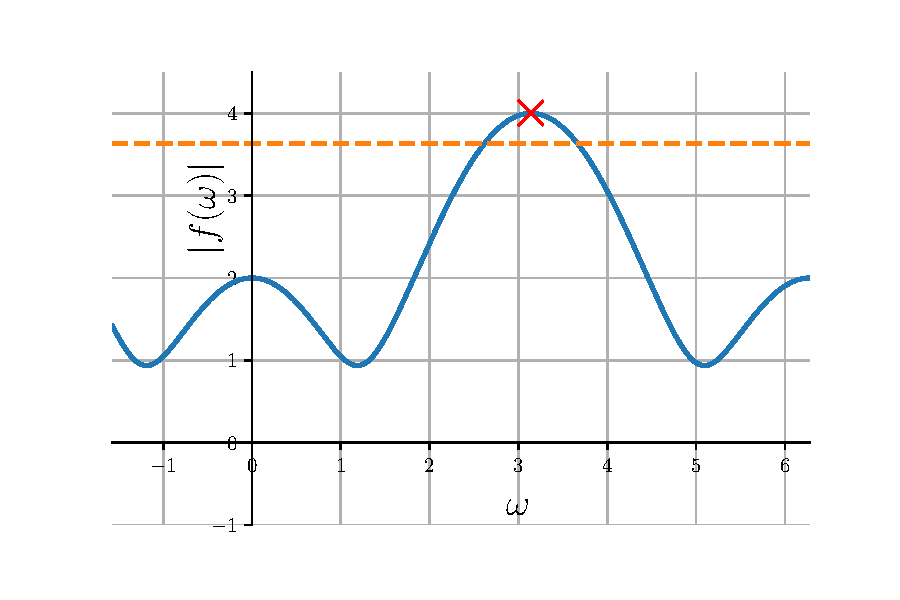
\includegraphics[scale=0.5]{images/graph_bound_gen_func/graph_n5.pdf}}\only<2>{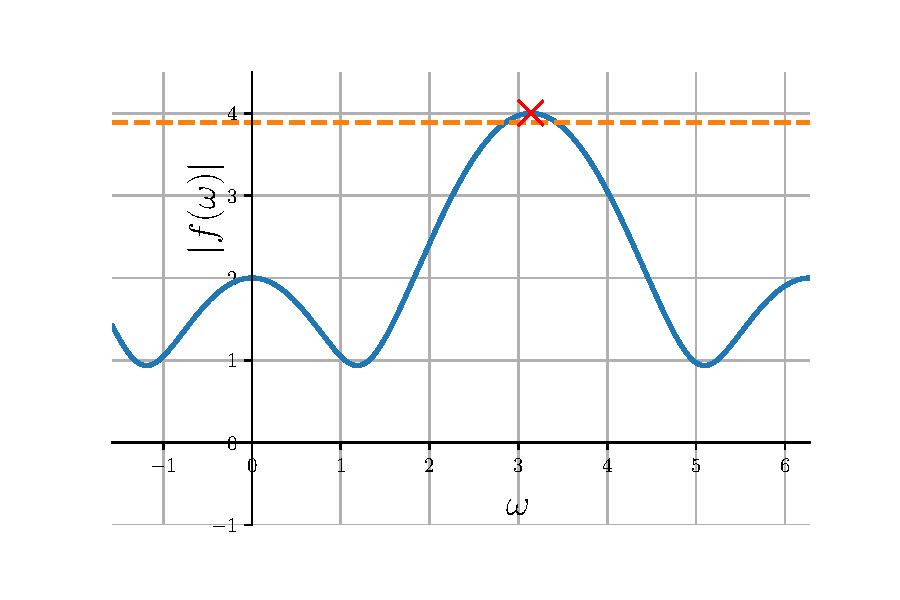
\includegraphics[scale=0.5]{images/graph_bound_gen_func/graph_n10.pdf}}\only<3>{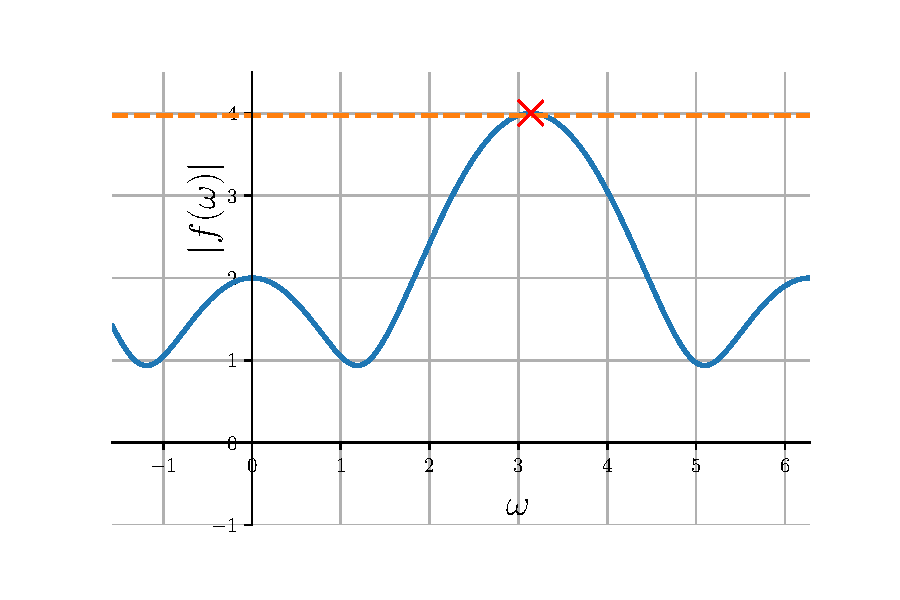
\includegraphics[scale=0.5]{images/graph_bound_gen_func/graph_n20.pdf}}
  \end{minipage}

  \def\point{10}
  \begin{tikzpicture}[overlay]
    \draw (9,3) node {{\color{darkblue}{$|f(\omega)|$}}};
    \visible<1>{  \draw (9.5,4.10) node {{\color{OrangePSL}{$\sigma_1(\Tmat) \approx 3.62$}}};}
    \visible<2>{  \draw (9.5,4.23) node {{\color{OrangePSL}{$\sigma_1(\Tmat) \approx 3.88$}}};}
    \visible<3->{ \draw (9.5,4.30) node {{\color{OrangePSL}{$\sigma_1(\Tmat) \approx 3.96$}}};}
  \end{tikzpicture}


\end{frame}





%%%%%%%%%%%%%%%%%%%%%%%%%%%%%%%%%%%%%%%%%%%%%%%%%%%%%%%%%%%%%%%%%%%%%%%%%%%%%%%
\begin{frame}{Equivalent Reasoning for Block Toeplitz Matrices}
%%%%%%%%%%%%%%%%%%%%%%%%%%%%%%%%%%%%%%%%%%%%%%%%%%%%%%%%%%%%%%%%%%%%%%%%%%%%%%%


  Let $g: [0, 2\pi] \rightarrow \Cbb^{m \times m}$ be a matrix-valued function and the inverse Fourier Transform of the sequence $\{ \Bsf_h \}_{\{-n+1, \dots, n-1\}}$:
  \begin{minipage}{\textwidth}
    \centering
    \begin{minipage}{0.45\textwidth}
      \begin{equation}
	  \Bmat = \scalebox{0.8}{
	  \begin{tikzpicture}[
	    baseline,
	    every left delimiter/.style={xshift=+0.78em},
	    every right delimiter/.style={xshift=-0.4em},
	    mymat/.style={
	      matrix of math nodes,
	      ampersand replacement=\&,
	      left delimiter=(,
	      right delimiter=),
	      nodes={
		text depth=0.5ex,
		text height=2ex,
		text width=2em,
		align=center}
	    }
	    ]
	    \matrix[mymat] (mytoeplitz) {
	       \Bsf_0  \& \Bsf_1 \& \cdots \& \Bsf_{n-1} \\
	       \Bsf_{-1} \& \color{black!30}{\Bsf_0} \& \color{black!30}{\ddots} \& \color{black!30}{\vdots} \\
	       \vdots  \& \color{black!30}{\ddots}  \& \color{black!30}{\Bsf_0}    \& \color{black!30}{\Bsf_1} \\
	       \Bsf_{-n+1} \& \color{black!30}{\cdots}  \& \color{black!30}{\Bsf_{-1}} \& \color{black!30}{\Bsf_0} \\
	    };
	  \end{tikzpicture}}
	  \phantom{ = \Amat}
      \end{equation}
    \end{minipage}
    \begin{minipage}{0.45\textwidth}
      \begin{equation}
	g(\omega) = \sum_{h = -n+1}^{n-1} \Bsf_h e^{\ci h \omega} 
      \end{equation}
    \end{minipage}
  \end{minipage}

  \begin{theorem}[{\color{SkyBlue}{\cite{gutierrez2012block}}}\xspace]
    Let $\Bmat$ a block Toeplitz matrix and $g$ the inverse Fourier transform of its associated sequence, then:
    \begin{equation}
      \sigma_1 \left( \Bmat \right) \leq \sup_{\omega \in [0, 2\pi]} \sigma_1 \left( g\left( \omega \right) \right)
    \end{equation}
  \end{theorem}

\end{frame}







%%%%%%%%%%%%%%%%%%%%%%%%%%%%%%%%%%%%%%%%%%%%%%%%%%%%%%%%%%%%%%%%%%%%%%%%%%%%%%%
\begin{frame}{Extension to Doubly-Block Toeplitz Matrices}
%%%%%%%%%%%%%%%%%%%%%%%%%%%%%%%%%%%%%%%%%%%%%%%%%%%%%%%%%%%%%%%%%%%%%%%%%%%%%%%

  \begin{minipage}{\textwidth}
    \centering
    We extend the reasoning to doubly-block Toeplitz matrices with \\ \orangebold{2d trigonometric polynomials}.
  \end{minipage}

  \vspace{0.3cm}
  \begin{itemize}
    \item[$\bullet$] <2-> The first dimension generates the block Toeplitz structure
    \item[$\bullet$] <3-> The second dimension generates the Toeplitz structure of each block
  \end{itemize}

  \vspace{0.5cm}
  \begin{overlayarea}{\textwidth}{2.8cm}
    \centering
    \only<2>{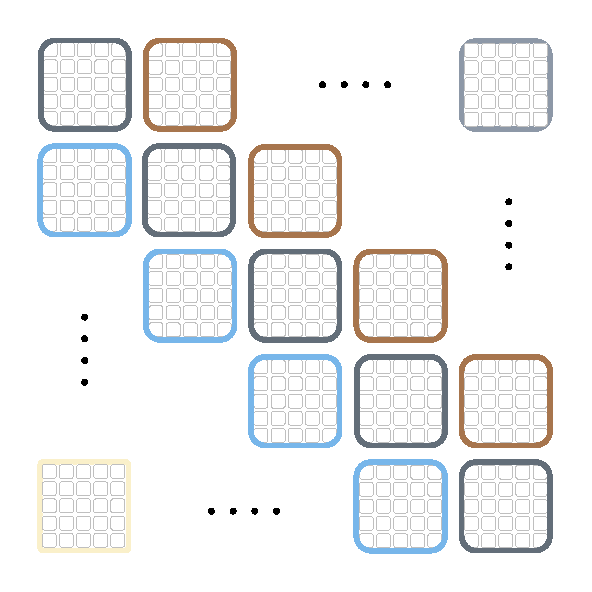
\includegraphics[scale=0.25]{images/doubly_block_v2.pdf}}\only<3->{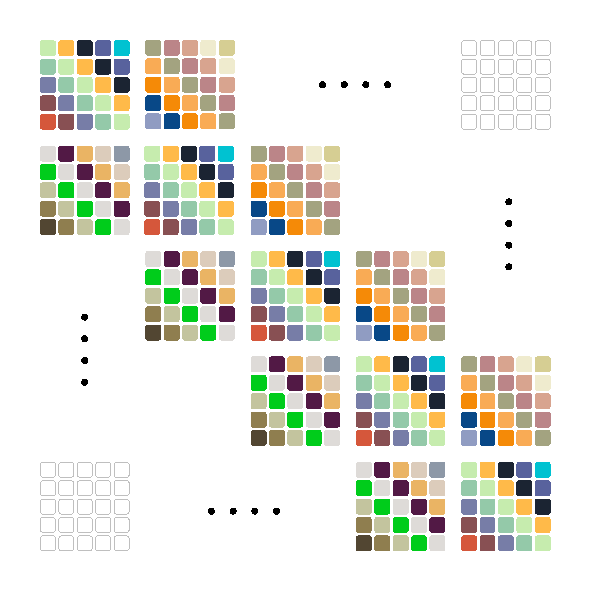
\includegraphics[scale=0.25]{images/doubly_block_v3.pdf}}
  \end{overlayarea}

\end{frame}




%%%%%%%%%%%%%%%%%%%%%%%%%%%%%%%%%%%%%%%%%%%%%%%%%%%%%%%%%%%%%%%%%%%%%%%%%%%%%%%
\begin{frame}{Bound on the Singular Values of Doubly-Block Toeplitz Matrices}
%%%%%%%%%%%%%%%%%%%%%%%%%%%%%%%%%%%%%%%%%%%%%%%%%%%%%%%%%%%%%%%%%%%%%%%%%%%%%%%

  In the same way as {\color{SkyBlue}{\cite{gray2006toeplitz}}}, we can bound the singular values of doubly-block Toeplitz matrices with their associated function.

  \visible<2->{
    \begin{theorem}[Bound on the singular values of a Doubly-Block Toeplitz]
      Let $\Dmat$ be a doubly-block Toeplitz matrix and $f$ its associated function, then:
      \vspace{-0.2cm}
      \begin{equation}
	\sigma_1 \left( \Dmat \right) \leq \sup_{\omega_1, \omega_2 \in [0, 2\pi]^2} |f(\omega_1,\omega_2)|
      \end{equation}
      \vspace{-0.2cm}
    \end{theorem}
  }

  \begin{itemize}
    \item[$\bullet$] <3-> Let $\phi$ be a convolution layer and $\Wmat$ the doubly-block Toeplitz equivalent to the convolution
    \item[$\bullet$] <4-> Let $f$ be the function associated with the matrix $\Wmat$
    \item[\orange{$\rightarrow$}] <5-> Then, we can upper bound the Lipschitz constant of the convolution:
      \begin{equation}
        \lip(\phi) \leq \sigma_1(\Wmat) \leq \sup_{\omega_1, \omega_2 \in [0, 2\pi]^2} |f(\omega_1,\omega_2)|
      \end{equation}
   \end{itemize}


\end{frame}


% %%%%%%%%%%%%%%%%%%%%%%%%%%%%%%%%%%%%%%%%%%%%%%%%%%%%%%%%%%%%%%%%%%%%%%%%%%%%%%%
% \begin{frame}{Convolution as Matrix-Multiplication}
% %%%%%%%%%%%%%%%%%%%%%%%%%%%%%%%%%%%%%%%%%%%%%%%%%%%%%%%%%%%%%%%%%%%%%%%%%%%%%%%
%   
%   % In practice, images has multiple \textbf{channels} (\eg RGB). We refer to the number of input channels $\cin$ and the number of output channels $\cout$.
%   In practice, images has multiple \textbf{channels}:
%   \vspace{-0.2cm}
%   \begin{itemize}
%     \item[$\bullet$] Input channels (\eg, RGB)
%     \item[$\bullet$] Output channels (number of convolution performed on the image)
%   \end{itemize}
%   \vspace{0.2cm}
%
%   \begin{minipage}{\textwidth}
%     \centering
%     \begin{minipage}{0.4\textwidth}
%       \centering
%       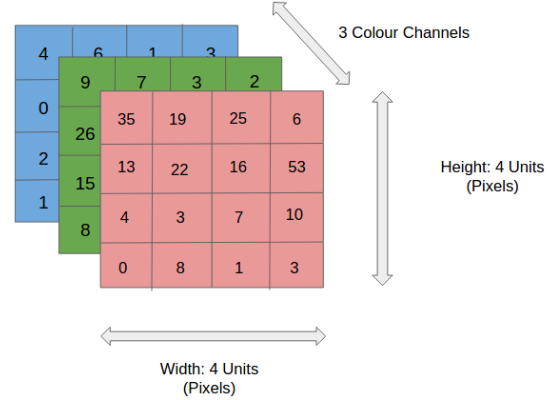
\includegraphics[scale=0.2]{images/image_rgb.png}
%     \end{minipage}
%     \begin{minipage}{0.4\textwidth}
%       \centering
%       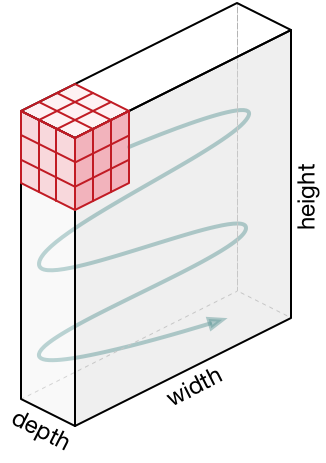
\includegraphics[scale=0.2]{images/conv_2d.png}
%     \end{minipage}
%   \end{minipage}
%
%   A multi-channel convolution is equivalent to a matrix-vector product where the matrix is a \textbf{block matrix} where each block is doubly-block Toeplitz matrix. 
%
% \end{frame}




%%%%%%%%%%%%%%%%%%%%%%%%%%%%%%%%%%%%%%%%%%%%%%%%%%%%%%%%%%%%%%%%%%%%%%%%%%%%%%%
\begin{frame}{Bound on the Singular Values of Convolution}
%%%%%%%%%%%%%%%%%%%%%%%%%%%%%%%%%%%%%%%%%%%%%%%%%%%%%%%%%%%%%%%%%%%%%%%%%%%%%%%
  

  \begin{minipage}{\textwidth}
    \centering
    \begin{minipage}{0.53\textwidth}
      In practice, images have multiple \textbf{channels}:
      {\small
      \begin{itemize}
	\item[$\bullet$] Input channels (\eg, RGB)
	\item[$\bullet$] Output channels (number of convolutions performed on the image)
      \end{itemize}
      }
    \end{minipage}
    \begin{minipage}{0.44\textwidth}
      \centering
      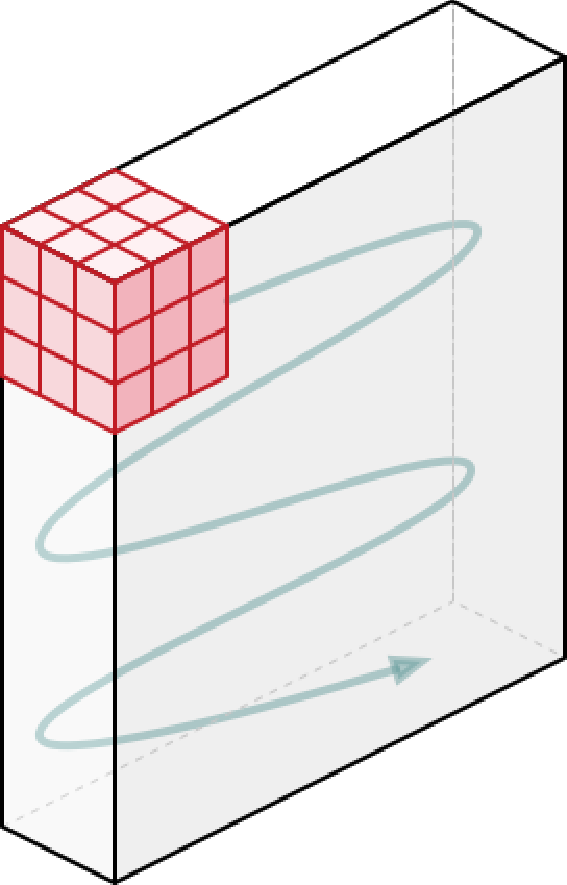
\includegraphics[scale=0.17]{images/conv_2d.pdf}
    \end{minipage}
  \end{minipage}


  \visible<2->{
    \begin{minipage}{\textwidth}
      \centering
      \begin{minipage}{0.49\textwidth}
	A multi-channel convolution is equivalent to a matrix-vector product where the matrix is a \textbf{block matrix} where each block is a doubly-block Toeplitz matrix. 
      \end{minipage}
      \begin{minipage}{0.49\textwidth}
	\centering
	\begin{equation}
	  \Mmat  = 
	    \scalebox{0.7}{
	    \begin{tikzpicture}[
	      baseline,
	      every left delimiter/.style={xshift=+0.78em},
	      every right delimiter/.style={xshift=-0.4em},
	      mymat/.style={
		matrix of math nodes,
		ampersand replacement=\&,
		left delimiter=(,
		right delimiter=),
		nodes={
		  text depth=0.5ex,
		  text height=2ex,
		  text width=3em,
		  align=center}
	      }
	      ]
	      \matrix[mymat] (matrix) {
		\Dmat_1\& \cdots \& \Dmat_{1,\cout} \\
		\vdots \& \& \vdots \\
		\Dmat_\cin \& \cdots \& \Dmat_{\cin,\cout} \\ 
	      };
	      \draw[decorate,decoration={mirror,raise=4pt},->] 
		($(matrix-1-3.north east)+(+0.4,0)$) -- node[above=4pt,sloped] 
		{Channels in}
		($(matrix-3-3.south east)+(+0.4,0)$);
	      \draw[decorate,decoration={mirror,raise=4pt},->] 
		($(matrix-1-1.north west)+(0,0.3)$) -- node[above=4pt,sloped] 
		{Channels out}
		($(matrix-1-3.north east)+(0,0.3)$);
	 \end{tikzpicture}}
	\end{equation}
       \end{minipage}
     \end{minipage}

    \begin{theorem}[Bound on the singular values of convolution]
      \begin{equation*}
	 \sigma_1(\Mmat) \leq \sqrt{ \sum_{i=1}^{\cout} \sup_{\omega_1, \omega_2 \in [0, 2\pi]^2} \sum_{j = 1}^{\cin} \left|f_{ij}(\omega_1, \omega_2) \right|^2 }  \triangleq \lipbound(\Mmat)
      \end{equation*}
    \end{theorem}
  }

\end{frame}






%%%%%%%%%%%%%%%%%%%%%%%%%%%%%%%%%%%%%%%%%%%%%%%%%%%%%%%%%%%%%%%%%%%%%%%%%%%%%%%
\begin{frame}{Tightness of LipBound}
%%%%%%%%%%%%%%%%%%%%%%%%%%%%%%%%%%%%%%%%%%%%%%%%%%%%%%%%%%%%%%%%%%%%%%%%%%%%%%%

  {\small
  \begin{itemize}
    \item[$\bullet$] The size of a matrix convolution is dependant on the size of the input
    \item[$\bullet$] When the size of the matrix increases, the associated function stays the same
  \end{itemize}
  }
  \vspace{-0.2cm}
  \begin{equation}
    \Gamma(n) = \lipbound(\Mmat(n)) - \sigma_1(\Mmat(n))
  \end{equation}
  \begin{minipage}{\textwidth}
    \centering
    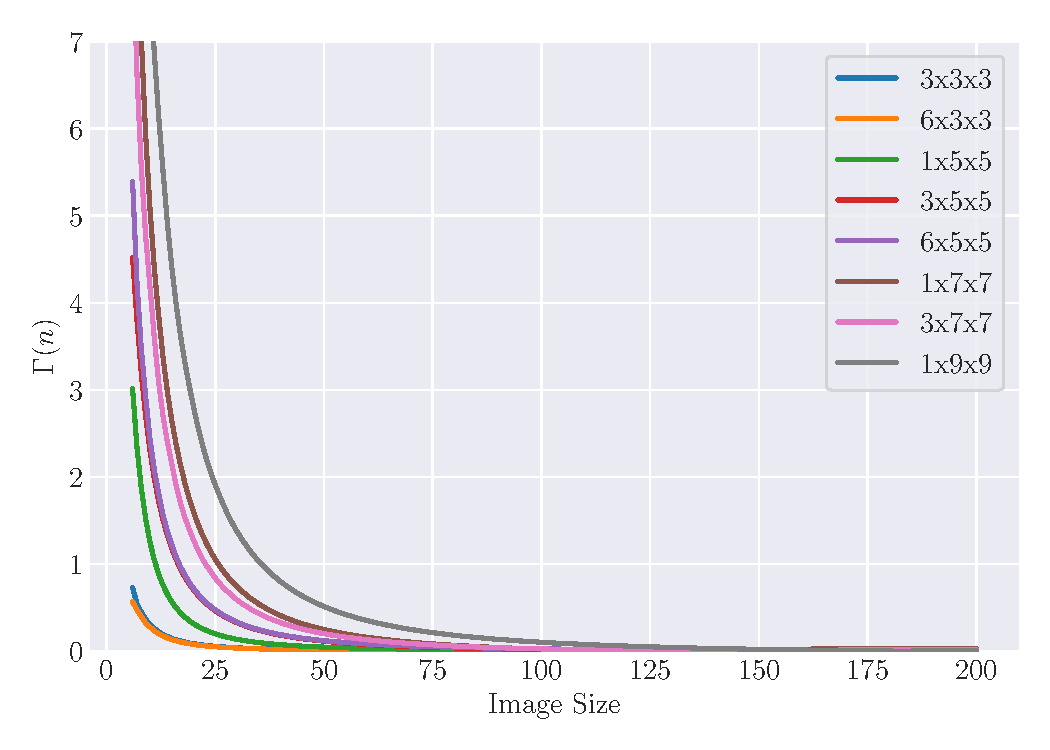
\includegraphics[scale=0.48]{images/convergence_bounds.pdf}
  \end{minipage}

\end{frame}


%%%%%%%%%%%%%%%%%%%%%%%%%%%%%%%%%%%%%%%%%%%%%%%%%%%%%%%%%%%%%%%%%%%%%%%%%%%%%%%
\begin{frame}{Computing LipBound}
%%%%%%%%%%%%%%%%%%%%%%%%%%%%%%%%%%%%%%%%%%%%%%%%%%%%%%%%%%%%%%%%%%%%%%%%%%%%%%%

  \begin{minipage}{\textwidth}
    \centering
    \begin{tabular}{cccc}
      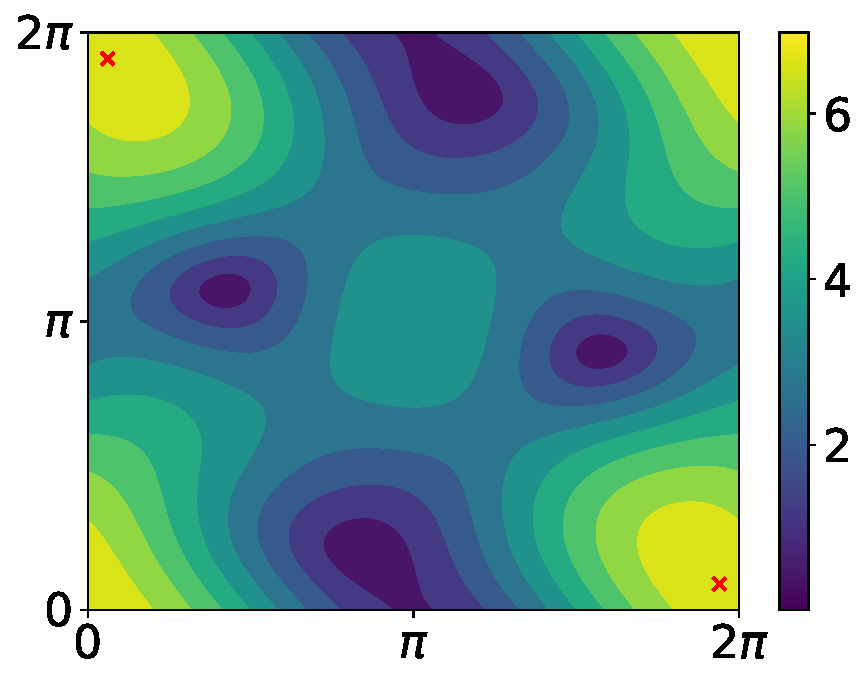
\includegraphics[scale=0.15]{images/contour_poly_200_1_1_3.pdf} &
      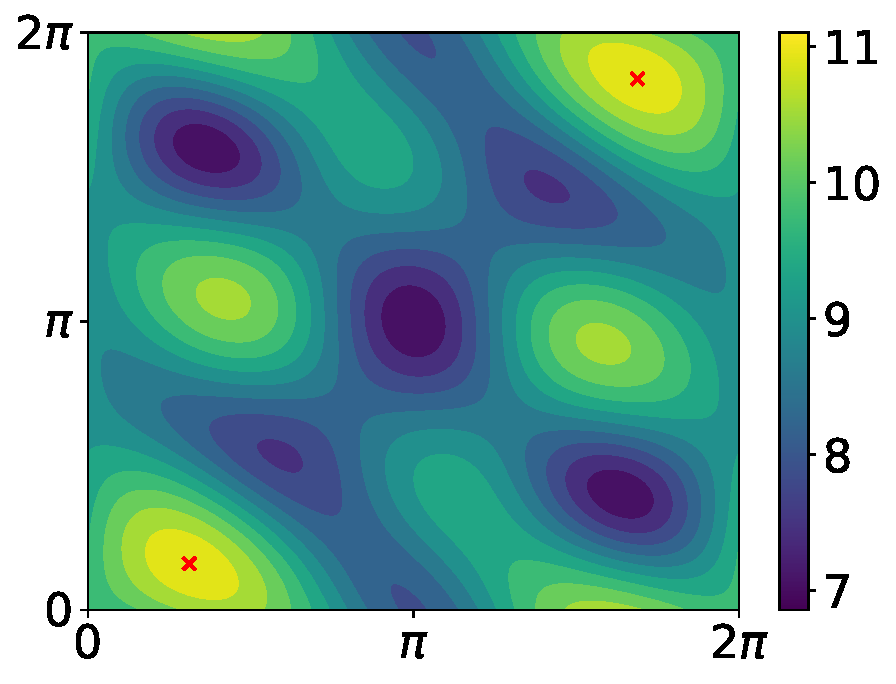
\includegraphics[scale=0.15]{images/contour_poly_200_1_9_3.pdf} & 
      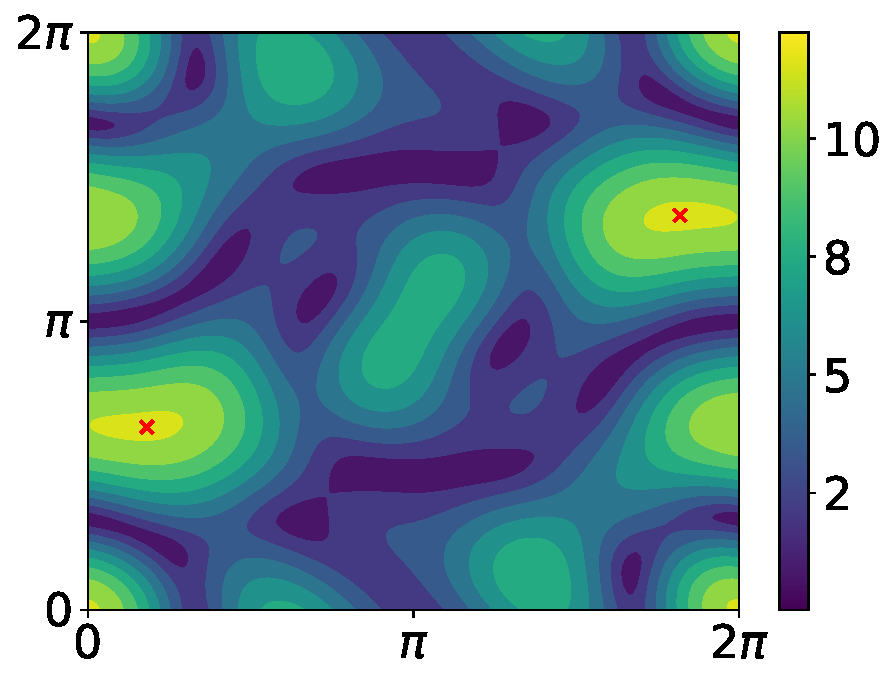
\includegraphics[scale=0.15]{images/contour_poly_200_1_1_5.pdf} & 
      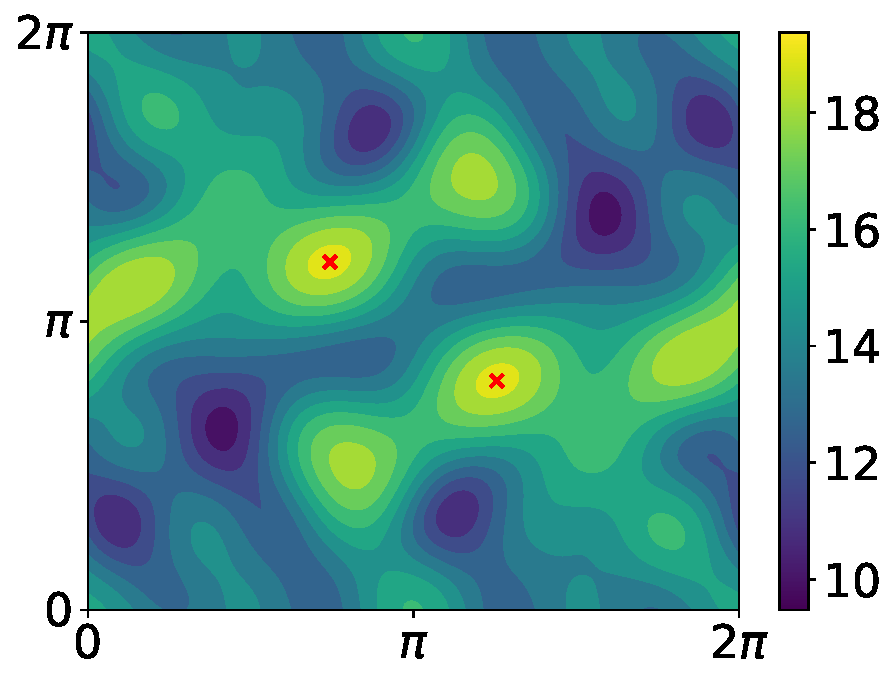
\includegraphics[scale=0.15]{images/contour_poly_200_1_9_5.pdf} \\
      \footnotesize{kernel $1\times3\times3$} &
      \footnotesize{kernel $9\times3\times3$} &
      \footnotesize{kernel $1\times5\times5$} &
      \footnotesize{kernel $9\times5\times5$}
    \end{tabular}

    \vspace{0.2cm}
    \footnotesize{Contour plot of multivariate trigonometric polynomials.}
  \end{minipage}

  \vspace{0.3cm}
  The computation of $\lipbound$ involves computing the maximum modulus of a 2-dimensional trigonometric polynomial on $[ 0, 2\pi]^2$.
  % Computing $\lipbound$ implies to compute the maximum modulus of a 2-dimensional trigonometric polynomial on 
  % $[ 0, 2\pi]^2$.

  \begin{itemize}
    \pause
  \item[$\bullet$] This problem has been known to be NP-hard ({\color{SkyBlue}{\cite{pfister2018bounding}}}).
    \pause
    \item[$\bullet$] However, trigonometric polynomials defined by usual convolutional kernels have a low degree (between 1 and 3)
    \pause
    \item[$\bullet$] A simple grid search algorithm is efficient and can be implemented on GPU
  \end{itemize}

\end{frame}


%%%%%%%%%%%%%%%%%%%%%%%%%%%%%%%%%%%%%%%%%%%%%%%%%%%%%%%%%%%%%%%%%%%%%%%%%%%%%%%
\begin{frame}{Precision of the Grid Search Algorithm}
%%%%%%%%%%%%%%%%%%%%%%%%%%%%%%%%%%%%%%%%%%%%%%%%%%%%%%%%%%%%%%%%%%%%%%%%%%%%%%%

  \begin{itemize}
    \item[$\bullet$] We can characterize the error of the grid search algorithm with respect to the number of samples $S$.
    \visible<2->{\item[$\bullet$] Let $f: [0, 2\pi]^2 \rightarrow \Cbb$ be a two dimensional trigonometric polynomial.}
  \end{itemize}

  \vspace{0.5cm}
  \begin{minipage}{\textwidth}
    \centering
    \begin{tabular}{ccc}
      \visible<2->{
      \begin{minipage}{0.2\textwidth}
	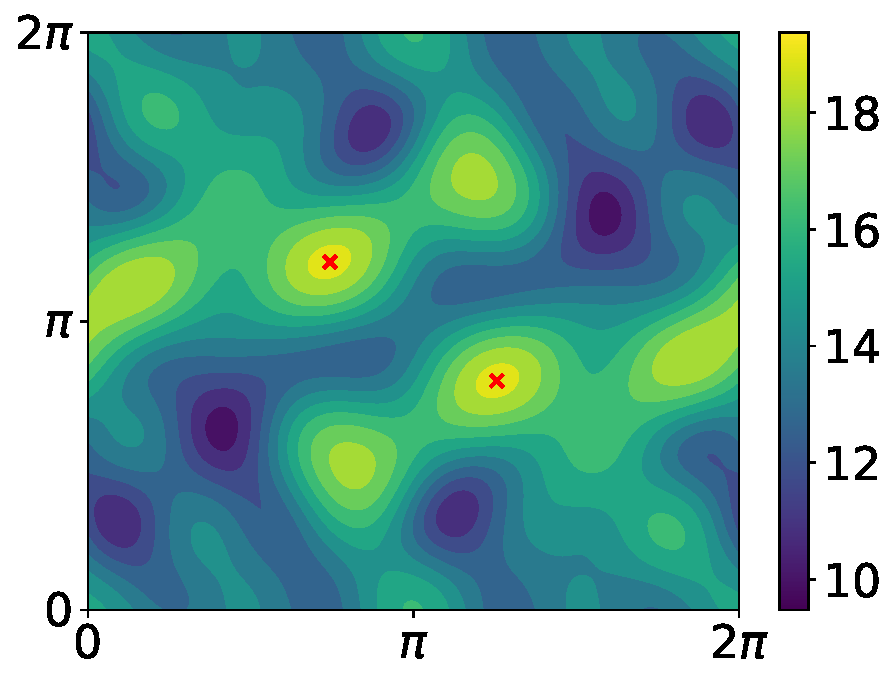
\includegraphics[scale=0.17]{images/contour_poly_200_1_9_5.pdf}
      \end{minipage}} & 
      \visible<3->{
      \begin{minipage}{0.2\textwidth}
	\centering
	$\underset{\text{discretization of}\atop\text{the search space}}{\Longrightarrow}$
      \end{minipage}} &
      \visible<3->{
      \begin{minipage}{0.2\textwidth}
	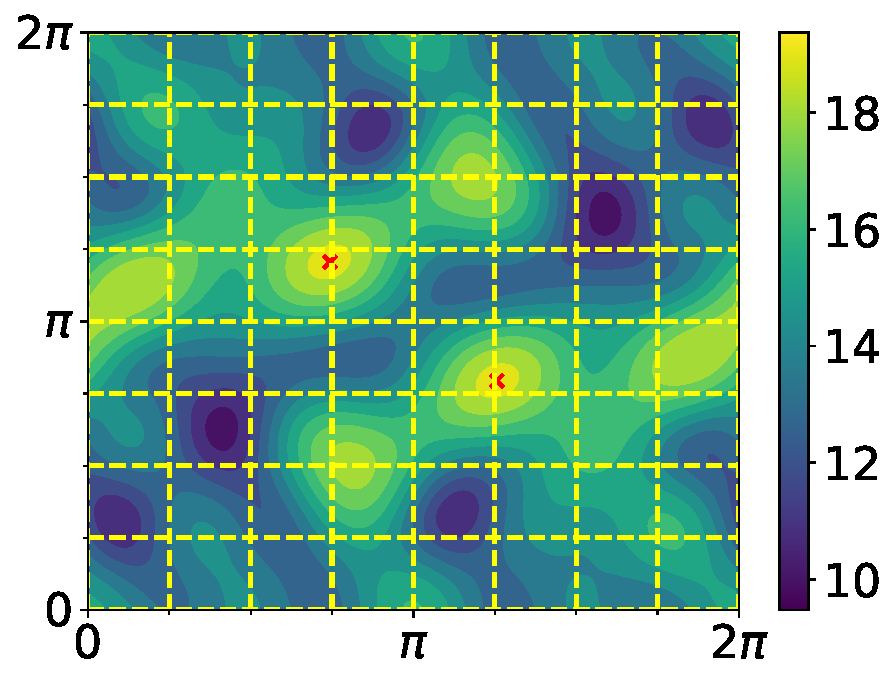
\includegraphics[scale=0.17]{images/contour_poly_200_1_9_5_grid.pdf}
      \end{minipage}} \\[1cm]
      \visible<2->{$\displaystyle \sup_{\omega_1, \omega_2 \in [0,2\pi]^2} \left| f(\omega_1, \omega_2) \right|$} & 
      \visible<4->{$\displaystyle \leq \frac{1}{(1 - \alpha)}$} &
      \visible<3->{$\displaystyle \max_{\omega_1', \omega_2' \in \Theta_S^2} \left| f(\omega_1', \omega_2') \right|$}
    \end{tabular}
  \end{minipage}

  \vspace{0.3cm}
  \visible<4->{
    \begin{itemize}
      \item where $\alpha = 2d/S$ is the degree of the polynomial \\
      \footnotesize{({\color{SkyBlue}{\cite{pfister2018bounding}}})}
    \end{itemize}
  }


\end{frame}



%%%%%%%%%%%%%%%%%%%%%%%%%%%%%%%%%%%%%%%%%%%%%%%%%%%%%%%%%%%%%%%%%%%%%%%%%%%%%%%
\subsection{Experiments}
%%%%%%%%%%%%%%%%%%%%%%%%%%%%%%%%%%%%%%%%%%%%%%%%%%%%%%%%%%%%%%%%%%%%%%%%%%%%%%%

% %%%%%%%%%%%%%%%%%%%%%%%%%%%%%%%%%%%%%%%%%%%%%%%%%%%%%%%%%%%%%%%%%%%%%%%%%%%%%%%
% \begin{frame}{Lipschitz Regularization of Convolutional Neural Networks}
% %%%%%%%%%%%%%%%%%%%%%%%%%%%%%%%%%%%%%%%%%%%%%%%%%%%%%%%%%%%%%%%%%%%%%%%%%%%%%%%
%  
%   We want to improve upon Adversarial Training:
%
%   \begin{equation}
%     \argmin_{h \in \Hcal} \ \frac{1}{m} \sum_{i = 1}^{m} \ell (h (\xvec_i + \tau^{\mathrm{adv}}(\xvec_i, y_i)), y_i) \color<1>{white}{ + \underbrace{{\color<3>{OrangePSL}{\lambda}} \sum_{j=1}^p \log(\lipbound(\Wmat^{(j)}))}_{\text{Our regularization}}}
%   \end{equation}
%
%   \visible<3->{
%     where {\color<3>{OrangePSL}{$\lambda$}} is user-defined parameter which controls the regularization.
%   }
%
%   \vspace{0.4cm}
%   \visible<4->{
%     $\Rightarrow$ Evaluation of the robustness with $l_2$ norm and several $\epsilon$
%   }
%
% \end{frame}


%%%%%%%%%%%%%%%%%%%%%%%%%%%%%%%%%%%%%%%%%%%%%%%%%%%%%%%%%%%%%%%%%%%%%%%%%%%%%%%
\begin{frame}{Lipschitz Regularization of Convolutional Neural Networks}
%%%%%%%%%%%%%%%%%%%%%%%%%%%%%%%%%%%%%%%%%%%%%%%%%%%%%%%%%%%%%%%%%%%%%%%%%%%%%%%
 
  We want to improve upon Adversarial Training:

  \begin{equation}
  \argmin_{h \in \Hcal} \ \frac{1}{m} \sum_{i = 1}^{m} \ell (h (\xvec_i + \tau^{\mathrm{adv}}(\xvec_i, y_i; h)), y_i)  + \underbrace{\lambda \sum_{j=1}^p \log(\lipbound(\Wmat^{(j)}))}_{\text{Our regularization}}
  \end{equation}
  where $\lambda$ is a user-defined parameter which controls the regularization.

  \vspace{0.4cm}
  $\Rightarrow$ Evaluation of the robustness with $l_2$ norm and several $\epsilon$

\end{frame}




% %%%%%%%%%%%%%%%%%%%%%%%%%%%%%%%%%%%%%%%%%%%%%%%%%%%%%%%%%%%%%%%%%%%%%%%%%%%%%%%
% \begin{frame}{Empirical Results}
% %%%%%%%%%%%%%%%%%%%%%%%%%%%%%%%%%%%%%%%%%%%%%%%%%%%%%%%%%%%%%%%%%%%%%%%%%%%%%%%
%
%   \begin{minipage}{\textwidth}
%     \centering
%     \small{
%     \begin{tabular}{lc}
%       \begin{tabular}{l}
% 	\orangebold{CIFAR10 Dataset $\quad$} \\
% 	50K images \\
% 	10 classes
%       \end{tabular}
%       &
%       \visible<2->{
%       \begin{tabular}{
% 	  M{l}{2-}
% 	  M{r}{2-}
% 	  M{r}{3-}
% 	  M{r}{4-}
% 	}
% 	\toprule
% 			   & \textbf{Accuracy}  & $\epsilon=0.6$ & $\epsilon = 0.8$ \\
% 	\midrule
%         \textbf{Baseline}  & \textbf{95}  & 0          & 0 \\
% 	\textbf{AT}        & 86           & 47          & 33 \\
% 	\textbf{AT+LipReg} & 80           & \textbf{54} & \textbf{43} \\
% 	\midrule
% 	  &  & +7 & +10 \\
% 	\bottomrule
%       \end{tabular}}
%      \end{tabular}
%      }
%   \end{minipage}
%
%
%
%   \vspace{0.8cm}
%   \visible<5->{
%   \begin{minipage}{\textwidth}
%     \centering
%     \small{
%      \begin{tabular}{lc}
% 	\begin{tabular}{l}
% 	  \orangebold{ImageNet Dataset $\quad$} \\
% 	  1.2M images \\
% 	  1000 classes
% 	\end{tabular}
%        &
%        \visible<6->{
%        \begin{tabular}{
% 	    M{l}{6-}
% 	    M{r}{6-}
% 	    M{r}{7-}
% 	    M{r}{8-}
%           }
% 	 \toprule
% 	   & \textbf{Accuracy} & $\epsilon=1$ & $\epsilon=2$ \\
% 	 \midrule
% 	 \textbf{Baseline}  & \textbf{78} & 0          & 0 \\
% 	 \textbf{AT}        & 50          & 30          & 16 \\
% 	 \textbf{AT+LipReg} & 51          & \textbf{33} & \textbf{20} \\
% 	 \midrule
% 	  & & +3 & +4 \\
% 	 \bottomrule
%        \end{tabular}}
%      \end{tabular}
%      }
%   \end{minipage}
%   }
%
% \end{frame}


%%%%%%%%%%%%%%%%%%%%%%%%%%%%%%%%%%%%%%%%%%%%%%%%%%%%%%%%%%%%%%%%%%%%%%%%%%%%%%%
\begin{frame}{Empirical Results}
%%%%%%%%%%%%%%%%%%%%%%%%%%%%%%%%%%%%%%%%%%%%%%%%%%%%%%%%%%%%%%%%%%%%%%%%%%%%%%%

  \begin{minipage}{\textwidth}
    \centering
    \small{
    \begin{tabular}{lc}
      \begin{tabular}{l}
	\orangebold{CIFAR10 Dataset $\quad$} \\
	50K images \\
	10 classes
      \end{tabular}
      &
      \begin{tabular}{lrrrr}
	\toprule
			   & \textbf{Accuracy}  & $\epsilon=0.6$ & $\epsilon = 0.8$ \\
	\midrule
        \textbf{Baseline}  & \textbf{95}  & 0          & 0 \\
	\textbf{AT}        & 86           & 47          & 33 \\
	\textbf{AT+LipReg} & 80           & \textbf{54} & \textbf{43} \\
	\midrule
	  &  & +7 & +10 \\
	\bottomrule
      \end{tabular}
     \end{tabular}
     }
  \end{minipage}



  \vspace{0.8cm}
  \visible<2->{
  \begin{minipage}{\textwidth}
    \centering
    \small{
     \begin{tabular}{lc}
	\begin{tabular}{l}
	  \orangebold{ImageNet Dataset $\quad$} \\
	  1.2M images \\
	  1000 classes
	\end{tabular}
       &
       \begin{tabular}{lrrr}
	 \toprule
	   & \textbf{Accuracy} & $\epsilon=1$ & $\epsilon=2$ \\
	 \midrule
	 \textbf{Baseline}  & \textbf{78} & 0          & 0 \\
	 \textbf{AT}        & 50          & 30          & 16 \\
	 \textbf{AT+LipReg} & 51          & \textbf{33} & \textbf{20} \\
	 \midrule
	  & & +3 & +4 \\
	 \bottomrule
       \end{tabular}
     \end{tabular}
     }
  \end{minipage}
  }

\end{frame}










  % %%%%%%%%%%%%%%%%%%%%%%%%%%%%%%%%%%%%%%%%%%%%%%%%%%%%%%%%%%%%%%%%%%%%%%%%%%%%%%%
\section{Conclusion \& Future Work}
%%%%%%%%%%%%%%%%%%%%%%%%%%%%%%%%%%%%%%%%%%%%%%%%%%%%%%%%%%%%%%%%%%%%%%%%%%%%%%%

%%%%%%%%%%%%%%%%%%%%%%%%%%%%%%%%%%%%%%%%%%%%%%%%%%%%%%%%%%%%%%%%%%%%%%%%%%%%%%%
\begin{frame}{Conclusion \& Future work}
%%%%%%%%%%%%%%%%%%%%%%%%%%%%%%%%%%%%%%%%%%%%%%%%%%%%%%%%%%%%%%%%%%%%%%%%%%%%%%%

 
  \begin{block}{Diagonal Circulant Neural Network}
  \begin{itemize}
    \item We proposed the use of a matrix decomposition into diagonal and circulant matrices in Deep Learning settings
    \item We applied have applied this structure for large scale video classification
    \item We showed that this method allows a good compression rate without an important impact on the accuracy. 
  \end{itemize}
  \end{block}

  \begin{block}{Lipschitz Bound of Convolutional Layers}
  \begin{itemize}
    \item We introduced a new bound on the Lipschitz constant of convolutional layers that is both accurate and efficient to compute;
    \item We used this bound to regularize the Lipschitz constant of neural networks;
    \item We showed that it increases the robustness of the trained networks to adversarial attacks;
  \end{itemize}
  \end{block}

\end{frame}

%%%%%%%%%%%%%%%%%%%%%%%%%%%%%%%%%%%%%%%%%%%%%%%%%%%%%%%%%%%%%%%%%%%%%%%%%%%%%%%
\begin{frame}{Lipschitz Regularization -- Limitation of the approach}
%%%%%%%%%%%%%%%%%%%%%%%%%%%%%%%%%%%%%%%%%%%%%%%%%%%%%%%%%%%%%%%%%%%%%%%%%%%%%%%

  % We can observe an increase in the robustness of the classifier with our Lipschitz Regularization. 
  % However, \textbf{we don't have any guarantee} that the global Lipschitz of the network is decreasing.

  Recent works (\cite{scaman2018lipschitz, NIPS2019_9319, latorre2020lipschitz}) have tried to devise algorithms to compute the Lipschitz constant of a Neural Network but these techniques are difficult to implement for neural networks with more than one or two layers.

  \begin{block}{Question}
   Can we leverage the block-Toeplitz structure of convolution to devise fast and accurate algorithm to compute the Lipschitz constant of Neural Networks ? 
  \end{block}


\end{frame}

% \begin{frame}{Tight bound of the global Lipschitz ?}
%
% It has been shown \citet{scaman2018lipschitz} that we can upper bound the global Lipschitz of a Neural Network as follows:
% \begin{equation}
%     \text{Lip}(\mathcal{N}) \leq
%   \max_{\forall i,\ \sigma_i \in [0, 1]^{n_i}} \norm{ \Wmat_\ell \text{diag}(\sigma_{\ell-1}) \Wmat_{k-1} \cdots \textrm{diag}(\sigma_1) \Wmat_1 }_2
% \end{equation}
%
% \paragraph{Question} Can we leverage the generating functions of doubly-block Toeplitz matrices to upper bound and compute the term:
%
% \end{frame}




  \section{Questions}

  \begin{frame}
    \centering
    \Huge Thank You
  \end{frame}

  % %%%%%%%%%%%%%%%%%%%%%%%%%%%%%%%%%%%%%%%%%%%%%%%%%%%%%%%%%%%%%%%%%%%%%%%%%%%%%%%
\section{Appendix}
%%%%%%%%%%%%%%%%%%%%%%%%%%%%%%%%%%%%%%%%%%%%%%%%%%%%%%%%%%%%%%%%%%%%%%%%%%%%%%%



%%%%%%%%%%%%%%%%%%%%%%%%%%%%%%%%%%%%%%%%%%%%%%%%%%%%%%%%%%%%%%%%%%%%%%%%%%%%%%%
\begin{frame}{Efficient Matrix-vector product with Circulant Matrices}
%%%%%%%%%%%%%%%%%%%%%%%%%%%%%%%%%%%%%%%%%%%%%%%%%%%%%%%%%%%%%%%%%%%%%%%%%%%%%%%

  A circulant matrix $\Cmat \in \Rbb^{n \times n}$ such as $\Cmat = \circulant (\cvec)$, with $\cvec \in \Rbb^n$ can be diagonalized by the Discrete Fourier Transform:
  \begin{equation*}
      \Cmat = \Wmat^{-1} \Lambda \Wmat
  \end{equation*}
  where 
  \begin{itemize}
    \item[$\bullet$] $\Wmat = \frac{1}{\sqrt{n}} \left( \omega^{jk} \right)_{j,k = 0, \dots, n-1}$ with $\omega$ being the $n^{th}$ root of unity
    \item[$\bullet$] $\Lambda$ is a diagonal matrix with the eigenvalues of the matrix $\Cmat$ which corresponds to $\Wmat \cvec$
  \end{itemize}

  Due to the convolution theorem, matrix-vector multiplication can be done efficiently with the \textbf{FFT} as follows:
  \begin{equation*}
    \Cmat \xvec = \mathrm{IDFT}( \mathrm{DFT}(\cvec) * \mathrm{DFT}(\xvec) )
  \end{equation*}

\end{frame}



%%%%%%%%%%%%%%%%%%%%%%%%%%%%%%%%%%%%%%%%%%%%%%%%%%%%%%%%%%%%%%%%%%%%%%%%%%%%%%%
\begin{frame}{Protecting Neural Networks against Several Types of Attacks}
%%%%%%%%%%%%%%%%%%%%%%%%%%%%%%%%%%%%%%%%%%%%%%%%%%%%%%%%%%%%%%%%%%%%%%%%%%%%%%%

  \begin{minipage}{\textwidth}
    \centering

    \scalebox{1}{
    \begin{tikzpicture}

      \foreach \PointA in {-5,-4,-3, -2,-1,0,+1,+2,+3,+4,+5} {
        \foreach \PointB in {0} {
	  \draw [fill=white,white,opacity=0] (\PointA,\PointB) circle (0.02cm);
	 }
      }

      \def\radiuscircle{2.4cm}
      \def\sizesquare{2cm}

      \draw plot[only marks,mark=x] coordinates{(-2, 0)};
      \node (image1)     at (-2, -0.2) {\footnotesize{image}};
      \node (circle1)    at (-2,  0.0) [draw, circle, minimum size=\radiuscircle] {};
      \node (rectangle1) at (-2,  0.0) 
        [draw, minimum width=\sizesquare, minimum height=\sizesquare, dashed] {};
      \draw[-latex] (-2,0) -- (-1.07,0.95);
      \draw plot[only marks,mark=x] coordinates{(-1.03,0.97)};

      \begin{scope}
	\color{red}
	\pgfsetlinewidth{0.5pt}
	\pgfsetplottension{0.9}
	\pgfplothandlercurveto
	\pgfplotstreamstart
	  \pgfplotstreampoint{\pgfpoint{-3.0cm}{+1.3cm}}
	  \pgfplotstreampoint{\pgfpoint{-1.11cm}{+0.89cm}}
	  \pgfplotstreampoint{\pgfpoint{-0.7cm}{-1.0cm}}
	\pgfplotstreamend
	\pgfusepath{stroke}
      \end{scope}

      \draw plot[only marks,mark=x] coordinates{(+2, 0)};
      \node (image2)     at (+2, -0.2) {\footnotesize{image}};
      \node (circle2)    at (+2,  0.0) [draw, circle, minimum size=\radiuscircle] {};
      \node (rectangle2) at (+2,  0.0) 
        [draw, minimum width=\sizesquare, minimum height=\sizesquare, dashed] {};
      \draw[-latex] (+2,0) -- (+2,1.12);
      \draw plot[only marks,mark=x] coordinates{(+2, 1.15)};

      \begin{scope}
	\color{blue}
	\pgfsetlinewidth{0.5pt}
	\pgfsetplottension{0.3}
	\pgfplothandlercurveto
	\pgfplotstreamstart
	  \pgfplotstreampoint{\pgfpoint{+1.0cm}{+1.1cm}}
	  \pgfplotstreampoint{\pgfpoint{+2.0cm}{+1.05cm}}
	  \pgfplotstreampoint{\pgfpoint{+3.05cm}{+1.05cm}}
	  \pgfplotstreampoint{\pgfpoint{+3.1cm}{-1.0cm}}
	\pgfplotstreamend
	\pgfusepath{stroke}
      \end{scope}

      \node (ball1)     at (-3.8, +1.2) {\footnotesize{$l_\infty$ ball}};
      \node (ball2)     at (-3.8, +0.0) {\footnotesize{$l_2$ ball}};
      \path[-latex] (ball1.south) edge [bend right] ($(rectangle1.north west)+(0.0,-0.1)$);
      \path[-latex] (ball2.south) edge [bend right] ($(circle1.west)+(0.0,0.0)$);

      \node (adv1)     at (-0.3, +1.3) {
        \begin{minipage}{0.2\textwidth}
          {\footnotesize
	    $l_\infty$ adversarial \\[-0.2cm] 
            example
          }
        \end{minipage}};

      \node (adv2)     at (+2.3, +1.5) {
        \begin{minipage}{0.2\textwidth}
          {\footnotesize
            $l_2$ adversarial \\[-0.2cm] 
            example
          }
        \end{minipage}};

      \node (model1) at (-3.9,2.0) {
	 {\footnotesize
        \begin{tabular}{c}
	  Model defended \\[-0.1cm] 
	  against $l_2$ attacks
        \end{tabular}}};

      \node (model2) at (+4.3,2.0) {
	{\footnotesize
        \begin{tabular}{c}
	  Model defended \\[-0.1cm] 
	  against $l_\infty$ attacks
         \end{tabular}}};

      \path[-latex] ($(model1.east)+(-0.3,+0.0)$) edge [bend left] (-2.5, 1.4);
      \path[-latex] (model2.south) edge [bend left] (3.1,1.1);

    \end{tikzpicture}}
  \end{minipage}


  \vspace{0.2cm}
  {\small
  \vspace{-0.2cm}
  \begin{itemize}
    \item[$\bullet$] Protecting against one type of attack does not protect against other types
    \item[$\bullet$] The volume of the intersection of the balls is negligible when $d$ is large
    \item[$\bullet$] It is necessary to mix defense strategies ({\color{SkyBlue}{\cite{araujo2020advocating,maini2020adversarial}}})
  \end{itemize} 
  }

  % {\small
  % \textbf{Perspective:}
  % \vspace{-0.2cm}
  % \begin{itemize}
  %   \item[$\bullet$] The largest singular value of matrix is the Lipschitz constant with respect to the $l_2$
  %   \item[$\bullet$] The Lipschitz constant can be defined with respect to other norms 
  %     % \begin{equation}
	% % \mathrm{Lip}_{p}(\phi) = \sup_{\substack{\xvec_1, \xvec_2 \in \Rbb^n \\ \xvec_1 \neq \xvec_2}} \frac{\norm{\phi(\xvec_1) - \phi(\xvec_2)}_p}{\norm{\xvec_1 - \xvec_1}_p}
  %     % \end{equation}
  %   \item[\orange{$\rightarrow$}] Improve the overall robustness with $l_p$ Lipschitz regularization
  % \end{itemize} 
  % }

\end{frame}




%%%%%%%%%%%%%%%%%%%%%%%%%%%%%%%%%%%%%%%%%%%%%%%%%%%%%%%%%%%%%%%%%%%%%%%%%%%%%%%
\begin{frame}{Empirical Results -- CIFAR-10 Dataset}
%%%%%%%%%%%%%%%%%%%%%%%%%%%%%%%%%%%%%%%%%%%%%%%%%%%%%%%%%%%%%%%%%%%%%%%%%%%%%%%

  \begin{block}{Dataset: CIFAR-10}
  \begin{itemize}
    \item 50K images
    \item 10 classes
  \end{itemize}
  \end{block}

  \begin{table}[t]
    \centering
      {\small
      \begin{tabular}{lrrrr}
      \toprule
      & \textbf{Accuracy} & \textbf{PGD}-$l_\infty$ 0.03 & \textbf{C\&W}-$l_2$ 0.6 & \textbf{C\&W}-$l_2$ 0.8 \\
      \midrule
      Baseline  & \textbf{95.3} & 0.00 & 0.02 & 0.00 \\
      AT        & 86.4 & 42.6 & 47.7 & 33.4 \\
      AT+LipReg & 80.8 & \textbf{45.7} & \textbf{54.7} & \textbf{43.8} \\
      \midrule
       & -5.6 & +3.1 & +7.0 & +10.4 \\
      \bottomrule
      \end{tabular}%
      }
    \caption{This table shows the Accuracy under $\ell_2$ and $\ell_\infty$ attacks of CIFAR10 dataset. We use $\lambda$ equals to $0.008$.}
  \end{table}%

\end{frame}


%%%%%%%%%%%%%%%%%%%%%%%%%%%%%%%%%%%%%%%%%%%%%%%%%%%%%%%%%%%%%%%%%%%%%%%%%%%%%%%
\begin{frame}{Empirical Results -- ImageNet Dataset}
%%%%%%%%%%%%%%%%%%%%%%%%%%%%%%%%%%%%%%%%%%%%%%%%%%%%%%%%%%%%%%%%%%%%%%%%%%%%%%%

  \begin{block}{Dataset: ImageNet}
  \begin{itemize}
    \item 1,2 millions images
    \item 1000 classes
  \end{itemize}
  \end{block}

  \begin{table}[htbp]
    \centering
     {\small
       \begin{tabular}{lrrrr}
       \toprule
	 & \multicolumn{1}{l}{\textbf{Accuracy}} & \multicolumn{1}{c}{\textbf{PGD-}$l_\infty$ 0.02} & \multicolumn{1}{l}{\textbf{C\&W-}$l_2$ 1} & \multicolumn{1}{l}{\textbf{C\&W-}$l_2$ 2} \\
       \midrule
       Baseline  & \textbf{78.6} & 0.00 & 0.00 & 0.00 \\
       AT & 50.9 & 25.1 & 30.7 & 16.8 \\
       AT+LipReg & \textbf{51.9} & \textbf{25.9} & \textbf{33.8} & \textbf{20.4} \\
	\midrule
	 & +1.0 & +0.8 & +3.1 & +3.6 \\
       \bottomrule
       \end{tabular}%
       \caption{This table shows the accuracy and accuracy under attack of ImageNet dataset with different training schemes. We use $\lambda$  equal to $0.01$}
     }
  \end{table}%


\end{frame}








% %%%%%%%%%%%%%%%%%%%%%%%%%%%%%%%%%%%%%%%%%%%%%%%%%%%%%%%%%%%%%%%%%%%%%%%%%%%%%%%%
% \begin{frame}{Adversarial attacks}
% %%%%%%%%%%%%%%%%%%%%%%%%%%%%%%%%%%%%%%%%%%%%%%%%%%%%%%%%%%%%%%%%%%%%%%%%%%%%%%%%
%
%   \begin{minipage}{\textwidth}
%    \centering
%    An \textbf{adversarial attack} refers to a small change of an input maliciously designed to fool the result of a neural network. 
%   \end{minipage}
%   \vspace{0.7cm}
%
%   \begin{minipage}{\textwidth}
%     \centering
%     \begin{overpic}[trim=0 1.2cm 0 0.3cm, clip, width=0.9\textwidth]{images/ExampleAdversarialCatDog.pdf}
%       \put (7.5, 19) {
% 	\footnotesize Image
%       }
%       \put (39.5, 19) {
% 	\footnotesize Adversarial Perturbation
%       }
%       \put (78, 19) {
% 	\footnotesize Adversarial Image
%       }
%       \put (3.5, -3) {
% 	\footnotesize Label = ``cat''
%       }
%       \put (80, -3) {
% 	\footnotesize Label = ``dog''
%       }
%     \end{overpic}
%   \end{minipage}
%
%   \vspace{0.15cm}
%   \begin{itemize}
%     \item[$\bullet$] \orangebold{Numerous} methods exist to craft an \orangebold{adversarial perturbation};
%     \item[$\bullet$] The best attacks reduce the accuracy of an undefended model to \orangebold{0\%};
%   \end{itemize}
%
%   \vspace{0.5cm}
%   \begin{mdframed}[linecolor=OrangePSL,linewidth=1pt]
%     \centering
%     Adversarial examples poses a growing societal problem as more and more machine learning models are deployed into critical-decision systems.
%   \end{mdframed}
%
% \end{frame}


  \section{References}
  \begin{frame}[noframenumbering, allowframebreaks]{References}
    \bibliography{bibliography}
    \bibliographystyle{plainnat}
    \textbf{Picture License:} Pictures and photos in slides xxx and xxx have been designed by xxx
  \end{frame}

\end{document}




